%%%%%%%%%%%%%%%%%%%%%%%%%%%%%%%%%%%%%%%%%%%%%%%%%%%%%%%%%%%%%%%
%% HKUST(GZ) Thesis LaTeX Template
%%
%% This template is adapted from the original HKUST Thesis LaTeX3
%% Template developed by HKFoggyU and contributors.
%%
%% Original project repository:
%% https://github.com/HKFoggyU/hkust-thesis
%%
%% Contributors to original template:
%% https://github.com/HKFoggyU/hkust-thesis/graphs/contributors
%%
%% This modified version is customized for
%% The Hong Kong University of Science and Technology (Guangzhou),
%% HKUST(GZ), to meet the formatting needs of RPG students at HKUST(GZ).
%%
%% You can access and use this template from:
%% - Overleaf: aaa
%% - GitHub:   bbb
%%
%% License:
%% LaTeX Project Public License (version 1.3c)
%%
%% DISCLAIMER:
%% The original and modified versions of this template are provided
%% without any guarantee of compliance with official thesis formatting
%% requirements. Please always refer to the latest RPG Handbook and
%% formatting guidelines provided by HKUST(GZ).
%%
%%%%%%%%%%%%%%%%%%%%%%%%%%%%%%%%%%%%%%%%%%%%%%%%%%%%%%%%%%%%%%%
\PassOptionsToPackage{giveninits=false}{biblatex}

\documentclass[
  %customlatinfont = windows,
  %custombibstyle = nature,
  displaycommittee = false,
  % blankpage = true,
]{hkustthesis}

%% Thesis information
\hkustsetup {
  %% Please wrap the items with {}.
  %% If one item is not applicable, just leave it {}.
  %% Please do not leave any blank lines without {}.
  info = {
    degree        = {mphil},  %% phd / mphil
    title         = {Multimodal Sensing-Assisted User Association and Tracking in Vehicular Networks},
    keywords      = {vehicular networks, user association, tracking, multimodal sensing},
    author        = {Yifeng YUAN},
    Hub           = {Information Hub},
    Thrust        = {IoT Thrust},
    program       = {Internet of Things},
    major         = {Internet of Things},
    supervisor    = {Shijian GAO},
    %% Co-supervisor; leave it {} if not available
    co-supervisor = {Jia YAN},
    submit-month  = {June 2026},      % <month year>
    submit-date   = {22 June 2025},   % <date month year>
    defend-date   = {20 July 2025},     % <date month year>
    depthead      = {Head of Thrust},
    %% reviewers only for some departments, like ECE
    reviewer      = {Prof. AAA (Chairperson), 
                     Prof. BBB (Supervisor),
                     Prof. CCC (Co-Supervisor),
                     Prof. DDD,
                     Prof. EEE,
                     Prof. FFF},
    reviewerdept  = {Artificial Intelligence Thrust,
                     AI Thrust,
                     AI Thrust,
                     AI Thrust,
                     AI Thrust,
                     Data Science and Analytics Thrust},
    reviewerext   = {Prof. FFF (External Examiner),
                     Department of HH\\{University of UU, at VV}},
    % reviewerext   = {},
    city          = {Guangzhou},
  }
}

%% Import extra packages
% \usepackage{indentfirst, xspace, xcolor}

%% Add custom command
% \newcommand{\todo}[1]{\textcolor{red}{TODO: #1}}
\newcommand{\eg}{\textit{e.g.}, }
\newcommand{\ie}{\textit{i.e.}, }

%% Set the specific author in bold style.
%% See https://tex.stackexchange.com/a/304968
%% Need to set `author+an = {n=highlight}` for your n-th authorship in bib file.
%% See more examples in the PDF manual.
\renewcommand*{\mkbibnamegiven}[1]{\ifitemannotation{highlight}{\textbf{#1}}{#1}}
\renewcommand*{\mkbibnamefamily}[1]{\ifitemannotation{highlight}{\textbf{#1}}{#1}}
%% The bib file for `List of Publications`
\addbibresource{mythesis_LoP.bib}

%% Import bib file for bibliography
\addbibresource{mythesis.bib}

\begin{document}

%% -------------------------------------------------
%% Thesis structure: In the order of
%% -------------------------------------------------
%% Titlepage  -> Authorization -> Signature ->
%% Acknowledgements ->
%% TOC -> List of Figures -> List of Tables ->
%% Abstract -> 
%% -------------------------------------------------
%% <Main body> -> 
%% -------------------------------------------------
%% References -> (Appendices)
%% -------------------------------------------------

\frontmatter
\maketitle 

%% Revision to the Guidelines on Thesis Preparation [w.e.f. Spring 2024/25]
%% Abstract should be positioned immediately after the Title page
\begin{abstract}
Vehicular networks operating at millimetre-wave and other high-frequency bands
require accurate and timely beam management, yet repeated beam sweeping can
consume substantial radio resources in dynamic road environments. This thesis
develops a Distributed Multimodal Sensing-Assisted Beam Management framework,
denoted by DMSA-BM, for user association and tracking in vehicular networks.
The base-station-centric setting combines
multiview cameras at the serving base station (BS), multiview cameras at distributed
sensing nodes, and a BS-side point cloud derived from integrated sensing and
communication (ISAC). These observations are fused in a bird's-eye-view (BEV)
representation to support vehicle detection, per-target beam prediction, and
selection of a set of \(K\) candidate beams. To bridge
sensing outputs and communication identities, the framework
uses channel state information reference signal (CSI-RS) measurements selected
consistently with their synchronisation signal block (SSB) parents for initial or renewed
target-to-user association and an interacting multiple-model filter to maintain
physical-target tracks. A system-level communication abstraction based on beam
training overhead, regularised zero-forcing precoding, downlink
signal-to-interference-plus-noise ratio (SINR), and
overhead-adjusted effective rate is introduced to evaluate how
sensing, association, and tracking affect communication performance. The thesis
also defines a multimodal simulation and evaluation methodology that connects
road traffic generation, multisensor observations, ray-tracing-based beam
labels, and communication metrics for vehicular networks.
\end{abstract}

\authorization
\signaturepage

\begin{acknowledgements}
TODO: Draft acknowledgements near the final submission stage.
\end{acknowledgements}



\tableofcontents
\listoffigures
\listoftables
% TODO: see \cmd{\newlistofalgorithms}
\newlistofalgorithms % This is to maintain the same appearance

%% Dedication and Preface are optional
%\input{chapters/Pre_Dedication.tex}
%\input{chapters/Pre_Preface.tex}

%% -------------------------------------------------
%% Main body
%% -------------------------------------------------
\mainmatter

\chapter{Introduction}
\label{ch:introduction}

\section{Background}
\label{sec:introduction-background}

Vehicular networks are becoming an important part of connected mobility, intelligent transportation systems, and future wireless infrastructure. In vehicle-to-infrastructure (V2I) communication, roadside base stations (BSs) are expected to provide high-rate and reliable links for vehicles whose positions, velocities, and blockage conditions vary rapidly over time. The use of millimetre-wave and other high-frequency bands can provide large communication bandwidth, but it also makes the communication link more dependent on narrow beams, accurate beam alignment, and timely beam maintenance \cite{xu2022computervisionaidedmmwave,jiang2022lidaraidedfuturebeam,liu2020radarassistedpredictivebeamformingvehicular}.

In conventional high-frequency cellular systems, beam management is commonly supported by beam sweeping, synchronization signal block (SSB) measurements, channel state information reference signal (CSI-RS) measurements, and subsequent channel state information (CSI) feedback. These mechanisms allow the BS and the user equipment to identify suitable transmit and receive beams and to support later precoding decisions. However, when the users are vehicles moving through dynamic road environments, the validity of a beam measurement can be short-lived. A beam that is suitable at one frame may become suboptimal after a short displacement, a lane change, or the emergence of a blockage. Performing frequent full beam sweeps can reduce this uncertainty, but it consumes time-frequency resources that would otherwise be used for data transmission \cite{alrabeiah2019millimeterwavebasestations,charan2021visionpositionmultimodalbeamprediction,charan2023camerabasedmmwavebeam}.

Roadside infrastructure also has a natural sensing role. A BS can be equipped with cameras and integrated sensing and communication (ISAC) capability, while nearby sensing nodes (SNs) can provide additional views of the road using distributed cameras. These sensing observations are not merely auxiliary context: they can reveal vehicle locations, motion patterns, occlusion relationships, and road geometry before or alongside communication measurements. In this thesis, the sensing infrastructure is treated as a source of spatial information that can assist beam management in a BS-centric vehicular network. The service BS collects its own multiview camera observations, its BS-side ISAC point cloud, and the multiview camera observations from nearby SNs. These inputs are then fused in a bird's-eye-view (BEV) representation to support vehicle detection and per-target beam prediction.

The central motivation is that beam management in vehicular networks should not be considered only as a communication measurement problem. If the network can identify which detected vehicle corresponds to which communication user, and if it can maintain this identity over time, sensing information can be used to narrow the beam search space and reduce the frequency of full beam sweeping. This motivates a joint workflow that couples multimodal sensing, target-user association, tracking, and system-level communication evaluation \cite{alrabeiah2019millimeterwavebasestations,demirhan2021radaraided6gbeam,jiang2022lidaraidedfuturebeam,liu2022learningbasedpredictivebeamformingintegrated}.

\section{Challenges}
\label{sec:introduction-challenges}

The first challenge is the fast temporal variation of the wireless link. In a road environment, a vehicle may change its relative angle and distance to the serving BS over a small number of frames. The received beam power distribution over a discrete BS codebook can therefore change quickly, particularly in high-frequency bands where narrow beams are used. A sensing-assisted system must predict useful candidate beams from visual and ISAC observations while accounting for the fact that the communication channel and the sensing scene are both time-varying.

The second challenge is blockage and measurement uncertainty. Vehicles, roadside objects, and surrounding infrastructure can occlude line-of-sight or dominant reflection paths. At the same time, sensing observations can be incomplete because of camera field-of-view limits, synchronization errors, calibration errors, or sparse ISAC point clouds. Communication measurements can also be noisy or outdated. A practical beam management workflow must therefore tolerate uncertain observations across both sensing and communication modalities rather than assuming that either side provides a perfect state estimate.

The third challenge is multi-vehicle identity ambiguity. A detected sensing target is not automatically a communication user identity. In a scene with multiple vehicles, the sensing network may output several target detections and several per-target beam distributions, while the communication system observes beam power spectra associated with communication users. The system must determine which detected target corresponds to which user before the predicted beams can be used for user-specific communication decisions. This target-user association problem is essential in multi-vehicle sensing-assisted beam management, but it is distinct from the beam index prediction problem itself \cite{charan2023camerabasedmmwavebeam,imran2024environmentsemanticcommunicationenabling,zhou2020trackingobjectspoints}.

The fourth challenge is maintaining association over time. Repeating a full SSB beam sweep at every frame can re-establish user-specific beam observations, but it increases overhead. Conversely, relying only on a previous association can lead to beam mismatch when the vehicle moves, when tracking drifts, or when the scene becomes occluded. This motivates a tracking mechanism that predicts the state of associated users, matches new BEV detections to existing tracks, and decides when additional communication measurement is needed. In this thesis, the tracking component is based on an interacting multiple model (IMM) filter that combines multiple vehicle-motion hypotheses for temporally continuous identity maintenance.

These challenges indicate that a sensing-assisted vehicular beam management system should be evaluated beyond Top-K beam accuracy alone. Incorrect association, tracking failure, beam mismatch, and beam training overhead can all affect the final communication performance. For this reason, this thesis connects sensing outputs to a simplified system-level communication evaluation that includes beam training overhead, zero-forcing (ZF) precoding, effective signal-to-interference-plus-noise ratio (SINR), spectral efficiency, and overhead-adjusted throughput.

\section{Research Objective}
\label{sec:introduction-objective}

The objective of this thesis is to develop and evaluate a BS-centric multimodal distributed sensing-assisted framework for low-overhead and trackable beam management in vehicular networks. The framework uses the service BS as the coordination point. For each decision frame, the BS collects its local multiview camera observations, its BS-side ISAC point cloud, and the multiview camera observations from a selected set of nearby SNs. These multimodal observations are fused in a BEV representation to detect vehicles and to predict a per-target beam power distribution over the BS beam codebook.

The thesis focuses on four connected tasks. The first task is BEV-based vehicle detection from multimodal distributed sensing observations. The second task is per-target beam prediction, where each detected vehicle is assigned a predicted beam power distribution and a set of Top-K candidate beams. The third task is target-user association, where the initial SSB beam sweep power spectrum of each communication user is matched with the predicted beam distribution of detected sensing targets. The fourth task is tracking-assisted beam maintenance, where associated users are maintained over subsequent frames by combining BEV detections with an IMM tracking state.

The communication objective is not to reproduce a complete 5G New Radio protocol stack. Instead, this thesis adopts a simplified and interpretable system-level abstraction. In this abstraction, sensing-assisted Top-K beam prediction can reduce beam training overhead when the correct beam is included in the candidate set, while an incorrect candidate set introduces a beam mismatch penalty that affects subsequent CSI or precoding decisions. The resulting effective SINR, spectral efficiency, and overhead-adjusted throughput are then used to study how sensing accuracy, association reliability, tracking continuity, and measurement overhead interact at the communication-system level.

The resulting study is methodological and system-oriented: it defines the sensing-to-communication workflow, specifies the association and tracking interface, and evaluates how beam prediction, identity maintenance, and communication overhead interact in the proposed vehicular setting.

\section{Contributions}
\label{sec:introduction-contributions}

This thesis is organized around three contributions.

\begin{enumerate}
    \item A BS-centric multimodal distributed sensing-assisted beam management framework is developed for vehicular networks. The framework uses the serving BS as the coordination point and fuses BS-side multiview camera observations, BS-side ISAC point clouds, and camera observations from nearby distributed SNs. The fused BEV representation supports vehicle target detection and per-target beam power distribution prediction, from which Top-K candidate beams are obtained for later beam management decisions.

    \item A target-user association and tracking workflow is designed for multi-vehicle sensing-assisted communication. During initial access, the workflow uses the SSB beam sweep power spectrum from the communication side and the predicted per-target beam distribution from the sensing side to associate detected sensing targets with communication user identities. In later frames, an IMM tracking module and BEV detection association are used to maintain user identity and support temporally continuous beam selection while reducing reliance on repeated full beam sweeping.

    \item A multimodal vehicular simulation system and system-level evaluation method are constructed to connect sensing outputs with communication metrics. The simulation workflow links road traffic generation, multisensor observation generation, scene reconstruction, ray-tracing-based channel generation, beam power labels, and simplified communication evaluation. The evaluation considers Top-K beam prediction, target-user association, tracking error, beam training overhead, beam mismatch penalty, ZF precoding SINR, spectral efficiency, and overhead-adjusted throughput.
\end{enumerate}

The contributions are stated at the framework, association-and-tracking, and system-evaluation levels; quantitative performance claims are made only where they are supported by the experimental evaluation.

\section{Thesis Organization}
\label{sec:introduction-organization}

The remainder of this thesis is organized as follows. Chapter~\ref{ch:background} reviews the background and related work on vehicular beam management, sensing-assisted beam prediction, ISAC predictive beamforming, BEV multimodal fusion, cooperative perception, target-user association, and tracking. It also identifies the research gap addressed by this thesis.

Chapter~\ref{ch:system-model} presents the system model and problem formulation. It defines the roadside vehicular network, BSs, distributed SNs, vehicle users, multimodal sensing observations, target-user association variables, tracking states, and the communication and beam management model used for system-level evaluation.

Chapter~\ref{ch:methodology} describes the proposed multimodal sensing-assisted beam management framework. It introduces the BS-centric data flow, BEV-based multimodal fusion, vehicle detection head, per-target beam prediction head, initial target-user association procedure, IMM tracking module, and the interface between sensing outputs and communication evaluation.

Chapter~\ref{ch:experiments} describes the multimodal simulation system and experimental evaluation. It covers scenario and dataset construction, baselines, evaluation metrics, main results, ablation studies, and discussion of limitations.

Finally, Chapter~\ref{ch:conclusion} concludes the thesis and discusses future work. It summarizes the findings supported by the thesis, clarifies the main limitations of the simulation and communication abstraction, and outlines possible extensions toward more realistic protocol-level simulation, robust multimodal sensing, and broader cooperative vehicular network settings.

\chapter{Background and Related Work}
\label{ch:background}

Chapter~\ref{ch:introduction} identified three requirements for sensing-assisted
vehicular beam alignment: distributed multimodal perception that can reveal
relevant physical targets, target-to-user association that assigns sensing
evidence to the correct communication entity, and a resource-aware evaluation
that determines whether the resulting beam-management policy is worthwhile.
This chapter reviews the literature through those requirements rather than as a
collection of disconnected sensing modalities or learning architectures. The
review first establishes the measurement burden in high-frequency V2I beam
management and the opportunity offered by sensing-aided beam prediction. It
then considers distributed multimodal BEV perception, target-to-user association
with temporal tracking, and system-level V2I evaluation. The chapter concludes
by positioning the three contributions of this thesis relative to the respective
boundaries of prior work.

\section{Beam Management and Sensing-Aided Beam Prediction}
\label{sec:background-beam-management}

\subsection{Measurement Burden in High-Frequency V2I Communication}
\label{subsec:background-codebooks-training}

High-frequency V2I communication relies on directional transmission to obtain
sufficient array gain. A BS consequently has to identify a beam that is suitable
for each active vehicle and revise that decision as vehicle geometry, visibility,
and propagation conditions evolve. In practical codebook-based systems, this
process is supported by initial-access sweeps, reference-signal measurements,
and later refinement. The measurements are valuable because they are tied
directly to the communication link, but they consume radio resources and become
less informative as the vehicle moves or the environment changes.

The resulting trade-off is especially acute on roads. Relative position changes
quickly, vehicles and roadside structures intermittently block dominant paths,
and several users may occupy similar angular sectors. A policy that measures a
large beam set frequently can maintain reliable link evidence, but it reduces
the resources available for data transmission. A policy that measures a small
set risks missing a useful beam or retaining stale channel information. This
relationship between beam-search cost and communication performance motivates
beam prediction as a candidate-reduction mechanism rather than as an isolated
classification task \cite{xu2022computervisionaidedmmwave,liu2020radarassistedpredictivebeamformingvehicular,liu2022learningbasedpredictivebeamformingintegrated}.

Evaluation of beam-management methods should therefore distinguish several
quantities. A beam-ranking metric indicates whether a short candidate list
contains a useful direction, whereas a resource metric records the measurements
required to obtain that list. Neither quantity alone describes the communication
consequence. The latter also depends on how the selected beam affects the
effective channel, how often additional recovery measurements are required, and
how the measurement resources are accounted for. This distinction is important
when interpreting the sensing-aided studies reviewed below.

\subsection{From Sensing-Aided Prediction to Candidate Reduction}
\label{subsec:background-sensing-aided-prediction}

Sensing-aided beam prediction exploits the fact that wireless propagation is
coupled to the physical scene. Early vision-aided work showed that cameras at a
BS can assist blockage prediction and beam selection \cite{alrabeiah2019millimeterwavebasestations}. Subsequent V2I studies used visual information to infer beam
alignment or beam-coherence behaviour for moving vehicles
\cite{xu2022computervisionaidedmmwave}. Position-assisted methods use coarse
geometric information, while radar- and LiDAR-aided methods use range, angular,
and motion cues that are more directly linked to vehicle geometry
\cite{charan2021visionpositionmultimodalbeamprediction,demirhan2021radaraided6gbeam,jiang2022lidaraidedfuturebeam}. These approaches demonstrate that environment
observations can reduce the search space that must be examined by communication
measurements.

The prediction target varies across this literature. Some methods select a
single beam index, whereas others return a ranked candidate list or estimate the
power associated with each codebook beam. A distributional output is particularly
useful for beam management because it exposes both the ordering of candidates
and the concentration of the model's evidence. It can support Top-\(K\) candidate
selection, confidence assessment, and a later decision about whether the
candidate list is safe to use. Common metrics include Top-\(K\) accuracy,
received-power loss, and beam-search overhead. The DeepSense 6G data collection
and its associated beam-prediction challenge helped establish these metrics for
multimodal sensing-and-communication studies \cite{alkhateeb2023deepsense6glargescalerealworld,charan2022multimodalbeampredictionchallenge}.

Recent work extends this direction through multimodal transformers, sequential
models, and decision-oriented beam-management strategies
\cite{tian2023multimodaltransformerswirelesscommunications,ghassemi2024multimodaltransformerreinforcementlearningbased,farzanullah2025beamselectionisacusing}. These studies strengthen the case for using rich
environmental context, but they also reveal an important modelling boundary.
The learning sample is often already associated with a particular communication
link, either through the data construction or through an available position
label. In a multi-vehicle road scene, however, a BS first observes physical
objects and only subsequently has to determine which object is the UE represented
by a communication measurement. A useful beam ranking is therefore necessary,
but not sufficient, for user-specific beam alignment.

\section{Distributed Multimodal BEV Perception for Joint Vehicle Detection and Beam Prediction}
\label{sec:background-distributed-bev-perception}

\subsection{BEV Representation and Multimodal Fusion}
\label{subsec:background-bev-fusion}

Bird's-eye-view perception provides a natural spatial interface for roadside
multimodal sensing. Perspective camera images can be transformed into a
ground-plane representation, while point-cloud features can be encoded in the
same coordinate frame. Once expressed in BEV, information from different views
and modalities can be fused before target-level reasoning is performed. The
Lift-Splat-Shoot formulation illustrated how features from arbitrary camera rigs
can be lifted and projected into a BEV representation \cite{philion2020liftsplatshootencoding}. BEVFusion further showed the value of using a shared BEV
space to combine camera and geometric sensing for multiple perception tasks
\cite{liu2024bevfusionmultitaskmultisensorfusion}.

These ideas are useful for vehicular communication because beam quality is
strongly related to the geometry between the target BS, the vehicle, and the
surrounding environment. A BEV feature map can encode a vehicle's position,
local context, and relative visibility in the same representation from which
beam-related features are derived. Point-based detection methods such as
CenterNet offer an efficient way to represent vehicles by their centres and
associated attributes \cite{zhou2019objectspoints}. In a communication-oriented
extension, the target feature at a detected vehicle can also support prediction
of a beam-energy distribution. Thus, joint vehicle detection and beam prediction
need not be regarded as unrelated tasks: both depend on an accurate local scene
representation.

The transfer of BEV methods from autonomous driving to communication should,
however, be made carefully. Conventional BEV perception is commonly evaluated
through detection, segmentation, or motion forecasting. These outputs do not
automatically yield a communication decision. In the present context, the value
of BEV fusion lies in generating target-level evidence that can support a later
beam-management procedure. The perception output remains associated with a
physical target; it does not itself provide a communication UE identity or
confirm the final service beam.

\subsection{Distributed Sensing and Multimodal Beam Prediction}
\label{subsec:background-distributed-perception}

Cooperative perception extends single-site sensing by combining observations
from multiple agents or infrastructure nodes. In road environments, distinct
viewpoints can enlarge coverage, reduce the impact of an individual occlusion,
and make the scene representation less dependent on one camera's field of view.
V2X-ViT, for example, studies feature fusion across heterogeneous V2X agents
and highlights issues such as pose error and asynchronous observations
\cite{xu2022v2xvitvehicletoeverythingcooperativeperception}. These issues are equally relevant when a target BS draws on
neighbouring sensing nodes, even though the target BS remains the local
communication decision point.

Distributed sensing-aided networking and multimodal beam prediction provide the
closest communication-oriented precedents. Imran \emph{et al.} use distributed
RGB sensing nodes to provide environment semantics for beam prediction
\cite{imran2024environmentsemanticcommunicationenabling}. Multimodal prediction
studies combine image, point-cloud, radar, or position information to exploit
their complementary strengths \cite{tian2023multimodaltransformerswirelesscommunications,orimogunje2026occlusionawaremultimodalbeamprediction,mollah2026multimodalsensingfusionmmwave}. Zeng \emph{et al.} further demonstrate the potential of a BEV-fusion
formulation for sequential multimodal beam prediction
\cite{zeng2026bevfusionbasedframeworksequential}. Together, these studies show
that multimodal and spatially distributed observations can improve the evidence
available for beam-related inference.

Their scopes nevertheless leave an opportunity for a target-BS-centered
formulation that jointly treats roadside perception and user-level beam
management. Distributed sensing studies often exchange visual semantics rather
than fusing multiview cameras and BS-local ISAC-like geometry in a shared local
BEV frame. BEV beam-prediction studies do not necessarily distinguish a detected
physical target from the communication UE that will later consume the beam hint.
The first contribution of this thesis addresses this interface by using
distributed multimodal BEV perception for joint vehicle detection and per-target
beam prediction. Its purpose is to produce a structured physical-target
representation, not to bypass the association and measurement stages required
for beam alignment.

\section{Target-to-User Association with IMM-Based Tracking}
\label{sec:background-target-user-association-tracking}

\subsection{From Physical Targets to Communication Users}
\label{subsec:background-target-user-association}

The association problem arises because perception and communication attach
identity to different objects. A perception module detects physical vehicles,
and a tracking system assigns them temporal track identifiers. A communication
system, by contrast, schedules UEs and obtains link measurements indexed by
their communication identities. These identities may correspond to the same
vehicle, but the correspondence is not observed directly by a sensing model.
The distinction becomes material whenever multiple vehicles are visible, a
vehicle is temporarily missed, or an inactive object resembles an active UE.

Multi-candidate beam-prediction research begins to address this ambiguity.
Charan \emph{et al.} consider camera-based prediction in multi-candidate V2I
scenarios and introduce transmitter identification as part of the problem
\cite{charan2023camerabasedmmwavebeam}. Distributed environment-semantic
communication likewise includes transmitter identification and object
association-based tracking \cite{imran2024environmentsemanticcommunicationenabling}. These studies establish that object-level inference cannot be assumed to be
user-level inference. They do not, however, fully resolve how a target-to-user
association should be anchored by communication measurements, maintained after
temporary perception failures, and evaluated through its downstream influence on
beam-management decisions.

Target-to-user association in this thesis is therefore defined as a user-level
data-association problem. Sensing supplies a target-level beam likelihood and
communication measurement supplies UE-level beam evidence. A one-to-one
assignment connects the two only when the evidence is compatible and otherwise
preserves a conventional communication path. This interpretation differs from
using an oracle identifier, a geometric label, or a transmitter class as a
substitute for association. It establishes the correspondence needed for a beam
hint to be used by the correct UE.

\subsection{IMM-Based Tracking and Association Persistence}
\label{subsec:background-imm-tracking}

Association must also persist over time. Tracking-by-detection methods associate
new observations with previous tracks using spatial proximity, motion
consistency, appearance, or learned displacement. CenterTrack exemplifies a
point-based formulation that jointly reasons about detection and temporal
association \cite{zhou2020trackingobjectspoints}. In vehicular communication,
state prediction is additionally valuable because an anticipated vehicle motion
can inform when a previously established beam relationship should be refreshed.

ISAC predictive-beamforming studies provide complementary evidence for this
temporal viewpoint. Radar-assisted and Bayesian approaches use sensing-derived
state information to predict future beamforming decisions
\cite{liu2020radarassistedpredictivebeamformingvehicular,yuan2020bayesianpredictivebeamformingvehicular}. Learning-based methods use historical channels or sensing observations to capture
temporal dynamics for predictive beamforming \cite{liu2022learningbasedpredictivebeamformingintegrated,liu2022deepclstmpredictivebeamforming,du2021integratedsensingcommunicationsv2i}. The common premise is that vehicle state evolves continuously even when a
communication measurement is intermittent.

An interacting multiple-model (IMM) tracker is suitable for this setting because
it combines motion hypotheses that describe different vehicle behaviours, such
as approximately constant motion and manoeuvring turns. Its role in the present
thesis is deliberately specific. The IMM tracker maintains the temporal
validity of an association between a perception track and a communication UE;
it does not infer a UE identity from visual appearance. When the predicted track
and a new detection cease to agree, the resulting loss of confidence is a reason
to invoke measurement-assisted re-association rather than to continue applying
an old beam hint. The second contribution of this thesis consequently joins
target-to-user association with IMM-based tracking as a single mechanism for
identity-consistent beam alignment.

\section{Multimodal V2I Simulation and 5G NR-Oriented Beam-Management Evaluation}
\label{sec:background-v2i-evaluation}

\subsection{Multimodal Data and System-Level Simulation}
\label{subsec:background-multimodal-data}

Evaluation of sensing-assisted communication requires observations and channel
information that can be related at the same decision epoch. Multimodal data
collections such as DeepSense 6G provide synchronised communication and sensing
records that support controlled beam-prediction studies
\cite{alkhateeb2023deepsense6glargescalerealworld}. Realistic simulation
frameworks offer a complementary route by combining road traffic, environmental
sensing, and wireless propagation models. For example, Park \emph{et al.}
consider a multimodal realistic simulation framework for resource-efficient
beam prediction \cite{park2025resourceefficientbeampredictionmmwave}. These
resources make it possible to inspect how perception errors and communication
measurements interact, rather than assessing a learning model only on isolated
labels.

The Multimodal V2I Simulator considered in this thesis is a system-level
evaluation environment built on existing multimodal V2I data assets. It does not
claim to regenerate all sensing or propagation assets. Instead, it organises the
available observations, trajectories, beam-quality labels, and channel-related
information into beam-management episodes centred on the serving BS. This scope
is sufficient to compare the consequences of different sensing-assisted policies
while keeping the underlying data and radio assumptions common across methods.

\subsection{Resource-Aware Beam-Management Evaluation}
\label{subsec:background-resource-evaluation}

The evaluation of a sensing-assisted policy should preserve the distinction
between a prediction and a communication decision. A high Top-\(K\) beam metric
indicates that a small candidate set may contain a useful beam, but it does not
establish whether the beam was associated with the right UE, whether the
candidate set was actually measured, or whether the saved resources improved
the user experience. Conversely, an evaluation that reports an achievable rate
without accounting for the reference-signal resources can conceal the cost of
maintaining the required channel knowledge.

ISAC and learning-based beam-management studies have examined communication
objectives such as received power, spectral efficiency, sum rate, regret, and
latency \cite{liu2022learningbasedpredictivebeamformingintegrated,Wang_2023,ghassemi2024multimodaltransformerreinforcementlearningbased,farzanullah2025beamselectionisacusing,mollah2026multimodalsensingfusionmmwave}. Such objectives are necessary but must be interpreted under a stated
measurement model. A 5G NR-oriented abstraction provides this discipline by
representing the distinct roles of initial access, beam refinement, candidate
measurement, and data transmission without claiming to reproduce every
protocol-level procedure. It allows policies to be compared under a common
accounting of measurement resources and under common physical-layer assumptions.

The third contribution of this thesis combines the Multimodal V2I Simulator with
such a 5G NR-oriented beam-management evaluation framework. The evaluation
traces the error chain from target availability and beam ranking, through
target-to-user association and IMM-based tracking, to candidate recall,
measurement overhead, effective rate, lower-tail rate, and outage. It therefore
does not presuppose that an improvement in perception accuracy automatically
produces an improvement in communication performance. Rather, it makes the
conditions under which sensing evidence yields a favourable rate--overhead
trade-off explicit.

\section{Research Positioning and Summary}
\label{sec:background-gap}

The reviewed literature establishes the components required for sensing-assisted
beam alignment, but typically examines them at different points in the
sensing-to-communication chain. Sensing-aided beam-prediction studies show that
camera, radar, LiDAR, position, and multimodal observations can reduce the
uncertainty of beam selection. BEV fusion and cooperative perception show how
multi-view and multi-agent observations can form a more complete spatial
representation. Multi-candidate prediction, object association, and predictive
beamforming show that identity and temporal state matter once several moving
vehicles share the scene. Finally, system-level communication studies establish
the importance of rate and resource objectives. The remaining task is to connect
these elements without assuming away the target-to-user association problem.

The first contribution of this thesis is positioned at the interface between
distributed multimodal perception and communication-oriented inference. It
uses a target-BS-centered BEV representation to jointly detect vehicles and
predict their beam-energy distributions, thereby producing target-level evidence
that can reflect complementary viewpoints and sensing modalities. The second
contribution addresses the identity interface left open by target-level
prediction. It uses communication-side evidence for target-to-user association
and IMM-based tracking to maintain that association over time, so that a beam
hint is evaluated as user-specific information rather than as an anonymous
object prediction.

The third contribution completes the chain at the system level. The Multimodal
V2I Simulator and 5G NR-oriented beam-management evaluation framework compare
candidate-measurement and fallback decisions under common data and resource
assumptions. This framing makes it possible to determine whether a beam hint is
not only plausible for a visible target but also correctly attributed, measured,
and beneficial for communication. The thesis is thus positioned as an
integration of distributed multimodal BEV perception, target-to-user association
with IMM-based tracking, and resource-aware beam-management evaluation. The
next chapter formalises the corresponding network entities, observations,
identities, and decision variables.

\chapter{System Model and Problem Formulation}
\label{ch:system-model}

This chapter defines the system model used throughout the thesis. The objective is
to provide a consistent notation for the vehicular network, the multimodal sensing
observations, the communication beam measurements, the target-user association
variables, and the simplified communication-performance abstraction. The model is
intended to support the sensing-assisted beam management framework developed in
the following chapter; it is therefore kept at a system level and avoids assuming
implementation details that have not yet been fixed.

\section{Network Scenario and Time Structure}
\label{sec:system-network-time}

We consider a roadside vehicular network consisting of base stations (BSs),
distributed sensing nodes (SNs), and mobile vehicle users. Let
\(\mathcal{B}\) denote the set of BSs. A BS provides downlink communication
service to vehicles in its local coverage region and also acts as the center of a
local sensing-assisted beam management process. Let \(\mathcal{S}_b\) denote the
set of SNs selected by BS \(b \in \mathcal{B}\) for cooperative sensing. The
number of cooperating SNs is denoted by \(K_{\mathrm{SN}}=|\mathcal{S}_b|\), and
is treated as a configurable system parameter rather than a fixed constant in
this first-pass formulation. Each SN contributes sensing observations but does
not directly provide communication service in the considered model.

The mobile communication users are vehicles traveling through the road region.
For a serving BS \(b\), the set of active vehicle users at decision epoch \(t\)
is denoted by \(\mathcal{U}_b(t)\). Each communication user corresponds to a
physical vehicle target in the sensing scene, but the sensing target identity and
the communication user identity are not assumed to be known a priori. This
distinction is central to the target-user association problem addressed in this
thesis.

Time is divided into discrete decision epochs \(t=0,1,\ldots,T-1\). Each epoch
may correspond to one sensing frame, one communication scheduling interval, or a
coarser beam-management interval depending on the final simulation setup. At
each epoch, BS \(b\) receives multimodal sensing observations from its local
sensor suite and from the cooperating SNs, maintains tracking states for
previously associated users, and selects a beam-management action for the active
vehicle users. Initial access epochs may include a more complete beam sweep,
whereas subsequent epochs are intended to rely more heavily on sensing-assisted
prediction and tracking.

Each BS and each SN is equipped with four tilted down-looking cameras that cover
the road region from multiple viewpoints. In addition, each BS has an ISAC
sensing capability that produces a local sensing point cloud. For BS \(b\), all
sensing inputs are represented in a local bird's-eye-view (BEV) coordinate frame
anchored to the BS or to a fixed road-side reference frame. The exact simulation
layout, the default value of \(K_{\mathrm{SN}}\), the frame duration, and the
spatial extent of the BEV region remain configuration choices.

TODO[unstable-method]: Fix the final BS/SN layout, the default number of
cooperative SNs, the frame duration, and the BEV coordinate range after the
simulation system is finalized.

\section{Multimodal Sensing Observation Model}
\label{sec:system-sensing-observation}

At epoch \(t\), BS \(b\) observes the road scene through camera and ISAC
modalities. The multiview camera observations at the BS are denoted by
\[
    \mathcal{I}_b(t)=\{I_{b,c}(t)\}_{c=1}^{4},
\]
where \(I_{b,c}(t)\) is the image captured by the \(c\)-th camera mounted on BS
\(b\). Similarly, the camera observations from the cooperating SNs are denoted
by
\[
    \mathcal{I}_{\mathcal{S}_b}(t)
    = \{I_{s,c}(t): s \in \mathcal{S}_b,\ c=1,\ldots,4\}.
\]
The BS-side ISAC modality is represented by a point-cloud observation
\[
    \mathcal{P}_b(t)=\{(\mathbf{q}_{b,m}(t), a_{b,m}(t))\}_{m=1}^{N_b^{\mathrm{pt}}(t)},
\]
where \(\mathbf{q}_{b,m}(t)\) denotes the three-dimensional location of the
\(m\)-th sensing point in the local coordinate system, \(a_{b,m}(t)\) denotes an
optional point attribute such as intensity or confidence, and
\(N_b^{\mathrm{pt}}(t)\) is the number of points available at epoch \(t\). This
point cloud is used as an
ISAC-like geometric observation and should not be interpreted as a fully
specified radar signal-processing model.

The complete sensing observation available to BS \(b\) is written as
\begin{equation}
    \mathcal{O}^{\mathrm{sen}}_b(t)
    = \left\{\mathcal{I}_b(t),\mathcal{I}_{\mathcal{S}_b}(t),\mathcal{P}_b(t)\right\}.
    \label{eq:sensing-observation}
\end{equation}
The camera images and point cloud are assumed to be temporally synchronized and
spatially calibrated before being fused. Let \(\mathcal{T}_{j \rightarrow b}\)
denote the calibrated transformation from the coordinate frame of sensor or node
\(j\) into the local BEV frame of BS \(b\). These transformations allow visual
features and ISAC point-cloud features to be encoded into a common BEV
representation. The detailed projection, lifting, and point-cloud encoding
operations are left to the method chapter, because their exact implementation is
still part of the model design.

After multimodal BEV fusion, a vehicle detection module outputs a set of detected
targets
\[
    \mathcal{D}_b(t)=\{d_{b,1}(t),\ldots,d_{b,N_b^{\mathrm{det}}(t)}(t)\}.
\]
For detected target \(d_{b,i}(t)\), the sensing-side target representation is
summarized as
\begin{equation}
    \mathbf{z}_{b,i}(t)
    = \left(\hat{\mathbf{p}}_{b,i}(t),\hat{\mathbf{l}}_{b,i}(t),
    \hat{c}_{b,i}(t)\right),
    \label{eq:target-representation}
\end{equation}
where \(\hat{\mathbf{p}}_{b,i}(t)=[\hat{x}_{b,i}(t),\hat{y}_{b,i}(t)]^{\mathrm{T}}\)
is the estimated BEV center, \(\hat{\mathbf{l}}_{b,i}(t)\) contains target-size
or box-related attributes when available, and \(\hat{c}_{b,i}(t)\) is a detection
confidence score. Additional attributes such as heading or appearance features
may be included if they are used by the final association and tracking modules.

TODO[unstable-method]: Specify the final BEV resolution, feature encoding,
camera-to-BEV projection, ISAC point-cloud representation, and detection-target
attributes after the network architecture is fixed.

\section{Communication and Beam Model}
\label{sec:system-communication-beam}

Each BS is equipped with a finite beam codebook for directional communication.
For BS \(b\), the codebook is denoted by
\[
    \mathcal{F}_b=\{\mathbf{f}_{b,1},\mathbf{f}_{b,2},\ldots,\mathbf{f}_{b,M_b^{\mathrm{beam}}}\},
\]
where \(\mathbf{f}_{b,m}\) is the \(m\)-th beamforming vector and
\(M_b^{\mathrm{beam}}\) is the codebook size. For a vehicle user
\(u \in \mathcal{U}_b(t)\), the channel from BS \(b\) at epoch \(t\) is denoted
by \(\mathbf{h}_{b,u}(t)\). The idealized beam quality of codebook beam \(m\) can
be expressed as
\begin{equation}
    g_{b,u,m}(t)
    = \left|\mathbf{h}_{b,u}^{\mathrm{H}}(t)\mathbf{f}_{b,m}\right|^2,
    \label{eq:beam-quality}
\end{equation}
up to a transmit-power and noise normalization. The vector
\(\mathbf{g}_{b,u}(t)=[g_{b,u,1}(t),\ldots,g_{b,u,M_b^{\mathrm{beam}}}(t)]\)
is referred to as the beam power distribution of user \(u\) with respect to the
codebook of BS \(b\).

The sensing-assisted beam prediction module does not directly know
\(\mathbf{g}_{b,u}(t)\), because its input is a detected sensing target rather
than a communication identity. For each detected target \(d_{b,i}(t)\), it
predicts a per-target beam quality vector
\begin{equation}
    \hat{\mathbf{g}}_{b,i}(t)
    = [\hat{g}_{b,i,1}(t),\ldots,\hat{g}_{b,i,M_b^{\mathrm{beam}}}(t)].
    \label{eq:predicted-beam-distribution}
\end{equation}
The predicted Top-\(K\) candidate beam set is then
\begin{equation}
    \hat{\mathcal{K}}_{b,i}(t)
    = \mathrm{TopK}_{K_{\mathrm{beam}}}\left(\hat{\mathbf{g}}_{b,i}(t)\right),
    \label{eq:topk-beams}
\end{equation}
where \(K_{\mathrm{beam}}\) denotes the number of candidate communication beams
retained for later beam management and evaluation. The notation
\(\mathrm{TopK}_{K_{\mathrm{beam}}}(\cdot)\) returns the indices of the
\(K_{\mathrm{beam}}\) largest entries in its argument.

During initial access, BS \(b\) may perform an SSB-like beam sweep for a
communication user \(u\). The resulting measurement is abstracted as a beam power
spectrum
\begin{equation}
    \mathbf{y}^{\mathrm{SSB}}_{b,u}(t_0)
    = [y^{\mathrm{SSB}}_{b,u,1}(t_0),\ldots,
       y^{\mathrm{SSB}}_{b,u,M_b^{\mathrm{beam}}}(t_0)],
    \label{eq:ssb-spectrum}
\end{equation}
where \(t_0\) is an initial access or re-association epoch. This measurement is
used to establish the correspondence between communication users and detected
sensing targets. In later epochs, the system may use only partial beam
measurements or calibration signals over a smaller candidate set, for example
over the predicted Top-\(K\) beams. Such measurements are modeled as auxiliary
communication observations rather than as a complete 5G NR protocol simulation.

This codebook-level abstraction is consistent with sensing-aided beam prediction
studies that supervise beam indices, Top-\(K\) candidate beams, or per-beam
quality distributions rather than modeling the complete standard-compliant
control procedure \cite{charan2021visionpositionmultimodalbeamprediction,alkhateeb2023deepsense6glargescalerealworld,charan2023camerabasedmmwavebeam,zeng2026bevfusionbasedframeworksequential}.

TODO[unstable-method]: Fix the final codebook size, beam-label generation
procedure, beam-power normalization, and abstraction of partial measurement or
calibration signals.

\section{Target-User Association and Tracking State}
\label{sec:system-association-tracking}

The system must connect three types of identity: detected sensing targets,
communication users, and temporal tracks. A detected target \(d_{b,i}(t)\)
describes an object observed in the BEV sensing output at epoch \(t\). A
communication user \(u\) is the network identity used for beam measurement,
scheduling, and throughput evaluation. A track \(r\) is a temporal state that
maintains the estimated motion of a physical vehicle across epochs.

Let \(a_{b,i,u}(t) \in \{0,1\}\) be the binary target-user association variable:
\begin{equation}
    a_{b,i,u}(t)=
    \begin{cases}
    1, & \text{if detected target } d_{b,i}(t) \text{ is associated with user } u,\\
    0, & \text{otherwise.}
    \end{cases}
    \label{eq:association-variable}
\end{equation}
The association is subject to one-to-one matching constraints at a given epoch,
\begin{equation}
    \sum_{u \in \mathcal{U}_b(t)} a_{b,i,u}(t) \leq 1,\quad
    \sum_{i=1}^{N_b^{\mathrm{det}}(t)} a_{b,i,u}(t) \leq 1.
    \label{eq:association-constraints}
\end{equation}
At an initial access epoch \(t_0\), the association may be estimated by matching
the sensing-predicted beam distribution \(\hat{\mathbf{g}}_{b,i}(t_0)\) with the
communication-side beam spectrum \(\mathbf{y}^{\mathrm{SSB}}_{b,u}(t_0)\), while
also considering BEV spatial priors and detection confidence when available. A
generic initial association problem can be written as
\begin{equation}
    \min_{\{a_{b,i,u}(t_0)\}}
    \sum_{i=1}^{N_b^{\mathrm{det}}(t_0)}
    \sum_{u \in \mathcal{U}_b(t_0)}
    a_{b,i,u}(t_0) C^{\mathrm{init}}_{b,i,u}(t_0),
    \label{eq:initial-association}
\end{equation}
subject to \eqref{eq:association-constraints}, where
\(C^{\mathrm{init}}_{b,i,u}(t_0)\) is an initial matching cost. In this thesis,
the cost is expected to include beam-spectrum similarity and may include
additional BEV-domain terms, but its final form is method-dependent.

For each associated vehicle, the system maintains a tracking state in the BEV
plane. Let \(r\) denote a track identity associated with a physical vehicle. A
minimal kinematic state is
\begin{equation}
    \mathbf{x}_{b,r}(t)
    = [x_{b,r}(t),y_{b,r}(t),v_{x,b,r}(t),v_{y,b,r}(t)]^{\mathrm{T}},
    \label{eq:tracking-state}
\end{equation}
where \((x_{b,r}(t),y_{b,r}(t))\) is the BEV position and
\((v_{x,b,r}(t),v_{y,b,r}(t))\) is the planar velocity. To support maneuvering
vehicles, the tracker may use an interacting multiple model (IMM) filter with a
set of motion models \(\mathcal{Q}\). The probability of motion model
\(q \in \mathcal{Q}\) for track \(r\) is denoted by \(\mu_{b,r,q}(t)\), with
\begin{equation}
    \sum_{q \in \mathcal{Q}} \mu_{b,r,q}(t)=1.
    \label{eq:imm-mode-probability}
\end{equation}
The IMM prediction provides a prior track state at epoch \(t\), which is then
associated with the new BEV detections \(\mathcal{D}_b(t)\). A generic
tracking-to-detection cost may be written as
\begin{equation}
    C^{\mathrm{trk}}_{b,r,i}(t)
    = \Psi_{\mathrm{trk}}\left(\hat{\mathbf{x}}^{-}_{b,r}(t),
    \mathbf{z}_{b,i}(t),\hat{\mathbf{g}}_{b,i}(t)\right),
    \label{eq:tracking-cost}
\end{equation}
where \(\hat{\mathbf{x}}^{-}_{b,r}(t)\) is the predicted track state before
measurement update and \(\Psi_{\mathrm{trk}}(\cdot)\) denotes a method-specific
association function. After a successful track-to-detection association, the
track state, the target-user mapping, and the beam prediction for the
corresponding communication user are updated jointly.

TODO[unstable-method]: Specify the final association cost, matching algorithm,
IMM motion models, gating thresholds, failure recovery rule, and whether beam
prediction is used directly in temporal association.

\section{Communication Performance Abstraction}
\label{sec:system-performance-abstraction}

The communication evaluation in this thesis uses a simplified and interpretable
system-level abstraction. It connects sensing-assisted Top-\(K\) beam prediction,
target-user association, tracking errors, and beam-management overhead to
multi-user communication metrics. It is not intended to reproduce the full 5G NR
protocol stack, detailed control-channel design, or exact standard-compliant
SSB/CSI-RS timing.

Let \(m_{b,u}(t)\) denote the selected beam index for user \(u\) served by BS
\(b\) at epoch \(t\). If the true effective beam for user \(u\) is contained in
the predicted candidate set associated with that user, the system can restrict
subsequent measurement or CSI acquisition to a smaller beam subset. If the
candidate set does not contain a sufficiently good beam, the selected beam and
the resulting CSI/PMI abstraction may be mismatched. We represent this effect
through a generic mismatch factor \(\eta_{b,u}(t)\), where larger values
correspond to more accurate beam and channel information.

For multi-user downlink evaluation, let \(\tilde{\mathbf{h}}_{b,u}(t)\) denote
the effective channel used by the evaluation module after the selected beam and
any mismatch abstraction have been applied. For a scheduled user set
\(\mathcal{U}^{\mathrm{sch}}_b(t) \subseteq \mathcal{U}_b(t)\), the BS forms a
ZF precoder
\begin{equation}
    \mathbf{W}_b(t)
    = [\mathbf{w}_{b,u}(t)]_{u \in \mathcal{U}^{\mathrm{sch}}_b(t)}
    \label{eq:zf-precoder}
\end{equation}
from the estimated or effective channel matrix. The resulting SINR of user \(u\)
is abstracted as
\begin{equation}
    \gamma^{\mathrm{ZF}}_{b,u}(t)
    =
    \frac{
    P_{b,u}(t)\left|\tilde{\mathbf{h}}_{b,u}^{\mathrm{H}}(t)
    \mathbf{w}_{b,u}(t)\right|^2
    }{
    \sum\limits_{v \in \mathcal{U}^{\mathrm{sch}}_b(t), v \neq u}
    P_{b,v}(t)\left|\tilde{\mathbf{h}}_{b,u}^{\mathrm{H}}(t)
    \mathbf{w}_{b,v}(t)\right|^2 + \sigma^2
    }.
    \label{eq:zf-sinr}
\end{equation}
Under perfect channel knowledge and feasible ZF, the inter-user interference
term is ideally suppressed. In the present abstraction, residual interference
may remain because sensing-assisted beam selection, target-user association, or
tracking errors can lead to imperfect effective-channel information.

The spectral efficiency of user \(u\) is then evaluated as
\begin{equation}
    r_{b,u}(t)=\log_2\left(1+\gamma^{\mathrm{ZF}}_{b,u}(t)\right).
    \label{eq:spectral-efficiency}
\end{equation}
Let \(\rho_{b,u}(t) \in [0,1]\) denote the fraction of the epoch consumed by
beam training, beam measurement, calibration, or re-association overhead for
user \(u\). The overhead-adjusted throughput is modeled as
\begin{equation}
    R^{\mathrm{adj}}_{b,u}(t)
    =
    \left(1-\rho_{b,u}(t)\right) B_b r_{b,u}(t),
    \label{eq:overhead-adjusted-throughput}
\end{equation}
where \(B_b\) is the bandwidth assigned by BS \(b\) in the simplified evaluation.
The system sum throughput at epoch \(t\) can be written as
\begin{equation}
    R^{\mathrm{sum}}_b(t)
    =
    \sum_{u \in \mathcal{U}^{\mathrm{sch}}_b(t)}
    R^{\mathrm{adj}}_{b,u}(t).
    \label{eq:sum-throughput}
\end{equation}
This abstraction allows the evaluation to account for two competing effects:
sensing-assisted prediction can reduce beam training overhead, while prediction,
association, or tracking failures can reduce the SINR through beam mismatch or
imperfect effective-channel estimation.

TODO[unstable-method]: Fix the mathematical mapping from Top-\(K\) beam miss,
beam mismatch, association failure, and tracking error to \(\eta_{b,u}(t)\) and
\(\tilde{\mathbf{h}}_{b,u}(t)\). Also fix the time or resource unit used to
compute \(\rho_{b,u}(t)\).

Similar system-level abstractions are commonly used in predictive beamforming
and ISAC studies to connect sensing, beam selection, and communication
performance through SINR, rate, or throughput-oriented metrics
\cite{liu2020radarassistedpredictivebeamformingvehicular,yuan2020bayesianpredictivebeamformingvehicular,liu2022learningbasedpredictivebeamformingintegrated,Wang_2023}.

\section{Problem Statement}
\label{sec:system-problem-statement}

Given the multimodal sensing observations
\(\{\mathcal{O}^{\mathrm{sen}}_b(t)\}_{t=0}^{T-1}\) and the communication
measurements available during initial access or later calibration, the system
aims to produce four coupled outputs. First, it detects vehicle targets in the
BEV frame. Second, it predicts a per-target beam power distribution and a
Top-\(K\) candidate beam set for each detected target. Third, it associates
detected sensing targets with communication user identities and maintains those
identities over time through tracking. Fourth, it evaluates the resulting
beam-management decisions through SINR, spectral efficiency, and
overhead-adjusted throughput under the simplified ZF-based communication model.

The problem can be summarized as the estimation and decision process
\begin{equation}
    \left\{\mathcal{O}^{\mathrm{sen}}_b(t),\mathbf{y}^{\mathrm{SSB}}_{b,u}(t_0),
    \mathcal{M}_{b,u}(t)\right\}
    \longrightarrow
    \left\{\mathcal{D}_b(t),\hat{\mathbf{g}}_{b,i}(t),
    \hat{\mathcal{K}}_{b,i}(t),a_{b,i,u}(t),
    \mathbf{x}_{b,r}(t),m_{b,u}(t)\right\},
    \label{eq:problem-mapping}
\end{equation}
where \(\mathcal{M}_{b,u}(t)\) denotes any later partial communication
measurement used for calibration or recovery. The desired behavior is to improve
beam prediction accuracy, maintain reliable target-user association and tracking,
reduce repeated full beam sweeps, and increase overhead-adjusted throughput. In
the current stage of the work, this objective is treated as a coupled
system-design and evaluation problem rather than as a single closed-form
optimization problem.

More formally, the final framework should balance the following goals:
accurate BEV target detection, high Top-\(K\) beam coverage, stable target-user
identity maintenance, low beam-management overhead, and high
\(R^{\mathrm{adj}}_{b,u}(t)\) under the evaluation model in
Section~\ref{sec:system-performance-abstraction}. The exact training losses,
matching costs, overhead accounting, and mismatch penalties will be specified
after the method and simulation pipeline are finalized.

TODO[unstable-method]: Convert this high-level problem statement into the final
mathematical formulation after the learning objectives, association cost,
tracking update, beam mismatch model, and evaluation protocol are fixed.

\chapter{Proposed Multimodal Sensing-Assisted Beam Management Framework}
\label{ch:methodology}

This chapter presents the proposed BS-centric multimodal sensing-assisted beam
management framework. The objective of the framework is to use distributed
sensing observations, initial communication measurements, and temporal tracking
to support vehicle detection, per-target beam prediction, target-user
association, and beam maintenance in vehicular networks. The chapter focuses on
the algorithmic data flow and system interface. It does not claim measured
performance improvement, because the experimental evidence and the final
simulation settings are not yet fixed.

\section{Framework Overview}
\label{sec:method-framework}

For each serving base station (BS), the proposed framework constructs a local
cooperative sensing region consisting of the BS itself and \(K_{\mathrm{SN}}\) neighbouring
sensing nodes (SNs). At decision epoch \(t\), the BS receives multiview camera
observations from its own cameras and the selected SN cameras, together with a
BS-side ISAC point cloud. During initial access or explicit calibration periods,
the BS also obtains communication-side beam measurements, such as an SSB beam
sweep power spectrum. The framework converts these heterogeneous observations
into a unified bird's-eye-view (BEV) representation and then performs four
coupled tasks:
\begin{enumerate}
  \item vehicle target detection in the BEV coordinate system;
  \item per-target beam power distribution prediction and Top-\(K\) candidate
        beam selection;
  \item initial target-user association using SSB-spectrum information; and
  \item tracking-assisted beam maintenance using an interacting multiple model
        (IMM) filter.
\end{enumerate}

Let \(\mathcal{C}_{b,t}\) denote the set of camera images available to BS
\(b\) at epoch \(t\), including the BS cameras and the cameras of the selected
SNs. Let \(\mathcal{P}_{b,t}\) denote the BS-side ISAC point cloud, and let
\(\mathcal{Y}_{b,t}\) denote the available communication measurements. The
overall mapping can be written abstractly as
\begin{equation}
  \left(
  \mathcal{D}_{b,t},
  \widehat{\mathcal{K}}_{b,t},
  \mathcal{A}_{b,t},
  \mathcal{X}_{b,t}
  \right)
  =
  \mathcal{G}_{\Theta}
  \left(
  \mathcal{C}_{b,t},
  \mathcal{P}_{b,t},
  \mathcal{Y}_{b,t},
  \mathcal{X}_{b,t-1}
  \right),
  \label{eq:method-overall-mapping}
\end{equation}
where \(\mathcal{D}_{b,t}\) is the set of detected BEV targets,
\(\widehat{\mathcal{K}}_{b,t}\) is the set of predicted Top-\(K\) beam
candidates for the detected or tracked targets, \(\mathcal{A}_{b,t}\) is the
target-user association state, and \(\mathcal{X}_{b,t}\) is the set of tracking
states. The parameter set \(\Theta\) represents the sensing network, detection
head, beam prediction head, and tracking-related parameters. A final framework
figure should show this data flow from multimodal input construction to the
communication evaluation interface.

The framework distinguishes between sensing target identity and communication
user identity. A detected vehicle in the BEV space is first a sensing target.
It becomes a communication user only after the system establishes a mapping
between the detection or track and a user identity observed by communication
measurements. This distinction is important in multi-vehicle scenes, where the
strongest predicted beam for a target does not by itself identify the user that
generated a communication-side beam spectrum.

\section{BEV-Based Multimodal Fusion}
\label{sec:method-multimodal-processing}

The sensing front end maps multiview camera observations and the BS-side ISAC
point cloud into a common BEV coordinate frame. The purpose of this BEV
representation is to align observations from different viewpoints, station
locations, and modalities before target detection and beam prediction are
performed. For BS \(b\), the camera feature extractor first transforms each
image \(I_{v,t} \in \mathcal{C}_{b,t}\) into an image-plane feature map. These
features are then projected or lifted into BEV coordinates using the available
calibration information:
\begin{equation}
  \mathbf{F}^{\mathrm{cam}}_{b,t}
  =
  \Phi_{\mathrm{cam}}
  \left(
  \{ I_{v,t}, \mathbf{T}_{v \rightarrow b} \}_{v \in \mathcal{V}_{b}}
  \right),
  \label{eq:method-camera-bev}
\end{equation}
where \(\mathcal{V}_{b}\) is the set of camera views used by BS \(b\), and
\(\mathbf{T}_{v \rightarrow b}\) denotes the calibration transform from camera
view \(v\) to the BS-centered BEV frame.

The ISAC point cloud is encoded into the same BEV frame through a point-cloud
encoder:
\begin{equation}
  \mathbf{F}^{\mathrm{isac}}_{b,t}
  =
  \Phi_{\mathrm{isac}}
  \left(
  \mathcal{P}_{b,t};
  \mathbf{T}_{\mathrm{isac} \rightarrow b}
  \right).
  \label{eq:method-isac-bev}
\end{equation}
The camera and ISAC BEV features are subsequently fused into a joint BEV feature
map,
\begin{equation}
  \mathbf{F}_{b,t}
  =
  \Phi_{\mathrm{fuse}}
  \left(
  \mathbf{F}^{\mathrm{cam}}_{b,t},
  \mathbf{F}^{\mathrm{isac}}_{b,t},
  \mathbf{M}_{b,t}
  \right),
  \label{eq:method-bev-fusion}
\end{equation}
where \(\mathbf{M}_{b,t}\) denotes optional modality-availability or confidence
masks. Such masks are useful because distributed sensing observations may be
missing, delayed, partially occluded, or noisy.

The current design assumes that temporal synchronization and spatial
calibration are handled before BEV fusion. In practice, calibration and
synchronization errors can affect both detection and beam prediction. Therefore,
the implementation should keep explicit records of sensor timestamps, camera
extrinsics, point-cloud coordinate transforms, and missing-modality indicators.
TODO[unstable-method]: Finalize the BEV grid resolution, coordinate range,
camera-to-BEV projection method, ISAC point-cloud encoding, feature fusion
strategy, and the treatment of missing or noisy sensing observations.

\section{Vehicle Detection and Per-Target Beam Prediction}
\label{sec:method-detection-beam}

The joint BEV feature map \(\mathbf{F}_{b,t}\) is processed by a CenterNet-like
detection head. Instead of proposing a large set of anchor boxes, the detection
head predicts a BEV heatmap whose local maxima correspond to vehicle centers.
For each BEV grid cell, the head may also predict center offsets, target size,
orientation-related attributes, and a detection confidence score. The detection
output is written as
\begin{equation}
  \mathcal{D}_{b,t}
  =
  \left\{
  d_{i,t}
  =
  \left(
  \widehat{\mathbf{p}}_{i,t},
  \widehat{\mathbf{s}}_{i,t},
  q_{i,t},
  \mathbf{e}_{i,t}
  \right)
  \right\}_{i=1}^{N_{b,t}},
  \label{eq:method-detection-output}
\end{equation}
where \(\widehat{\mathbf{p}}_{i,t}\) is the BEV center position,
\(\widehat{\mathbf{s}}_{i,t}\) denotes target attributes such as size, \(q_{i,t}\)
is the detection confidence, \(\mathbf{e}_{i,t}\) is the target-level feature
embedding, and \(N_{b,t}\) is the number of detected targets.

For each detected target, the beam prediction head estimates a distribution over
the BS beam codebook
\(\mathcal{F}_{b}=\{\mathbf{f}_{b,1},\ldots,\mathbf{f}_{b,M_b^{\mathrm{beam}}}\}\). The output
for target \(i\) is
\begin{equation}
  \widehat{\mathbf{g}}_{i,t}
  =
  \left[
  \widehat{g}_{i,t,1},
  \widehat{g}_{i,t,2},
  \ldots,
  \widehat{g}_{i,t,M_b^{\mathrm{beam}}}
  \right],
  \label{eq:method-beam-distribution}
\end{equation}
where \(\widehat{g}_{i,t,m}\) represents the predicted quality, normalized
power, or score of beam \(m\) for the detected target. The Top-\(K\) candidate
beam set is then defined as
\begin{equation}
  \widehat{\mathcal{K}}_{i,t}^{(K)}
  =
  \underset{
  \mathcal{S} \subseteq \{1,\ldots,M_b^{\mathrm{beam}}\},\ |\mathcal{S}|=K_{\mathrm{beam}}
  }{\operatorname{arg\,max}}
  \sum_{m \in \mathcal{S}} \widehat{g}_{i,t,m}.
  \label{eq:method-topk-beams}
\end{equation}
This distributional output is more informative than a single hard beam index:
it supports Top-\(K\) beam selection, uncertainty-aware association, and
communication-side mismatch modelling.

The training objective is expected to combine detection and beam-prediction
terms,
\begin{equation}
  \mathcal{L}
  =
  \lambda_{\mathrm{det}}\mathcal{L}_{\mathrm{det}}
  +
  \lambda_{\mathrm{beam}}\mathcal{L}_{\mathrm{beam}}
  +
  \lambda_{\mathrm{aux}}\mathcal{L}_{\mathrm{aux}},
  \label{eq:method-training-loss}
\end{equation}
where \(\mathcal{L}_{\mathrm{det}}\) may include heatmap, offset, and attribute
losses, \(\mathcal{L}_{\mathrm{beam}}\) supervises the predicted per-beam
distribution, and \(\mathcal{L}_{\mathrm{aux}}\) denotes optional auxiliary
terms. TODO[unstable-method]: Finalize the exact detection loss, beam
distribution loss, target-to-label assignment, positive and negative sample
definition, beam-label generation process, and beam power normalization.

\section{Initial Target-User Association}
\label{sec:method-association}

Initial target-user association is performed when communication-side beam
measurements are available. During initial access, the BS conducts an SSB beam
sweep and obtains a beam power spectrum for each communication user. Let
\(\mathbf{y}_{u,t_0}\) denote the observed spectrum for user \(u\) at the
initial association epoch \(t_0\):
\begin{equation}
  \mathbf{y}_{u,t_0}
  =
  \left[
  y_{u,t_0,1},
  y_{u,t_0,2},
  \ldots,
  y_{u,t_0,M_b^{\mathrm{beam}}}
  \right].
  \label{eq:method-ssb-spectrum}
\end{equation}
The sensing network simultaneously predicts
\(\widehat{\mathbf{g}}_{i,t_0}\) for each detected target \(i\). Association is
then formulated as a matching problem between detected sensing targets and
communication user identities.

A generic association cost can be expressed as
\begin{equation}
  c_{i,u}
  =
  \alpha_{\mathrm{beam}}
  d_{\mathrm{beam}}
  \left(
  \widehat{\mathbf{g}}_{i,t_0},
  \widetilde{\mathbf{y}}_{u,t_0}
  \right)
  +
  \alpha_{\mathrm{geo}}
  d_{\mathrm{geo}}(i,u)
  -
  \alpha_{\mathrm{conf}} q_{i,t_0},
  \label{eq:method-association-cost}
\end{equation}
where \(\widetilde{\mathbf{y}}_{u,t_0}\) is a normalized SSB spectrum,
\(d_{\mathrm{beam}}\) measures distributional disagreement,
\(d_{\mathrm{geo}}\) represents any available geometric prior, and \(q_{i,t_0}\)
is the detection confidence. The association variable is
\(a_{i,u,t_0} \in \{0,1\}\), where \(a_{i,u,t_0}=1\) means that sensing target
\(i\) is assigned to communication user \(u\). A one-to-one assignment can be
written as
\begin{equation}
  \begin{aligned}
  \min_{\{a_{i,u,t_0}\}} \quad
  & \sum_{i=1}^{N_{b,t_0}}\sum_{u=1}^{U_{b,t_0}}
    a_{i,u,t_0} c_{i,u} \\
  \mathrm{s.t.}\quad
  & \sum_{u=1}^{U_{b,t_0}} a_{i,u,t_0} \leq 1,\quad
    \sum_{i=1}^{N_{b,t_0}} a_{i,u,t_0} \leq 1, \\
  & a_{i,u,t_0} \in \{0,1\}.
  \end{aligned}
  \label{eq:method-initial-assignment}
\end{equation}
This formulation gives the intended interface without fixing the final cost
terms. TODO[unstable-method]: Finalize the association cost, spectrum
normalization, geometric prior, matching algorithm, conflict handling, rejection
thresholds, and recovery behaviour when no reliable one-to-one match exists.

Once a match is accepted, the framework creates a unified track containing a
sensing track identity, a communication user identity, a BEV state estimate, and
the current Top-\(K\) beam candidates. These associations are then maintained by
the tracking module rather than by repeated full beam sweeps at every epoch.

\section{IMM Tracking and Beam Maintenance}
\label{sec:method-tracking}

After initial association, the framework maintains each associated user through
an IMM tracking module. The tracking state for track \(\ell\) at epoch \(t\) is
represented as
\begin{equation}
  \mathbf{x}_{\ell,t}
  =
  \left[
  x_{\ell,t},
  y_{\ell,t},
  \dot{x}_{\ell,t},
  \dot{y}_{\ell,t}
  \right]^{\mathrm{T}},
  \label{eq:method-track-state}
\end{equation}
where \((x_{\ell,t},y_{\ell,t})\) is the BEV position and
\((\dot{x}_{\ell,t},\dot{y}_{\ell,t})\) is the BEV velocity. Additional
components, such as acceleration, heading, or lane-related state variables, can
be introduced if the final simulator and tracking design require them.

The IMM filter maintains a set of candidate motion models
\(\mathcal{Q}=\{1,\ldots,Q\}\). For each mode \(q \in \mathcal{Q}\), the predicted state is
abstractly written as
\begin{equation}
  \mathbf{x}^{(q)}_{\ell,t|t-1}
  =
  \mathbf{F}^{(q)}
  \mathbf{x}^{(q)}_{\ell,t-1|t-1},
  \qquad
  \mathbf{P}^{(q)}_{\ell,t|t-1}
  =
  \mathbf{F}^{(q)}
  \mathbf{P}^{(q)}_{\ell,t-1|t-1}
  \left(\mathbf{F}^{(q)}\right)^{\mathrm{T}}
  +
  \mathbf{Q}^{(q)}.
  \label{eq:method-imm-prediction}
\end{equation}
The mode-conditioned predictions are mixed according to the mode probabilities,
and the resulting predicted track is associated with the next-frame BEV
detections. If detection \(i\) provides measurement
\(\mathbf{z}_{i,t}=\widehat{\mathbf{p}}_{i,t}\), a generic tracking-association
score can include innovation distance, motion consistency, detection confidence,
and beam-distribution consistency:
\begin{equation}
  g_{\ell,i,t}
  =
  \beta_{\mathrm{pos}}
  d_{\mathrm{pos}}
  \left(
  \mathbf{z}_{i,t},
  \widehat{\mathbf{x}}_{\ell,t|t-1}
  \right)
  +
  \beta_{\mathrm{beam}}
  d_{\mathrm{beam}}
  \left(
  \widehat{\mathbf{g}}_{i,t},
  \widehat{\mathbf{g}}_{\ell,t-1}
  \right)
  -
  \beta_{\mathrm{conf}} q_{i,t}.
  \label{eq:method-track-detection-cost}
\end{equation}
The accepted detection updates the track state, refreshes the predicted beam
distribution, and propagates the communication user identity. If no reliable
detection is matched, the framework may keep a prediction-only track for a
limited duration and trigger a partial beam measurement or re-association
procedure.

Beam maintenance uses both the current beam prediction and the temporal
continuity encoded by the track. For a matched track \(\ell\), the communication
module receives the candidate set
\(\widehat{\mathcal{K}}_{\ell,t}^{(K)}\) from the associated detection. For a
temporarily unmatched track, the framework may use the predicted state and the
previous beam distribution as a short-term fallback, subject to confidence and
age limits. TODO[unstable-method]: Finalize the IMM motion-model set, mode
transition matrix, process and observation noise parameters, gating thresholds,
track birth and deletion rules, prediction-only lifetime, and the exact trigger
for partial beam measurement or re-association.

\section{Communication Interface and System-Level Evaluation}
\label{sec:method-communication-interface}

The communication interface receives, for each associated user \(u\), a user
identity, a tracking state, and a Top-\(K\) candidate beam set. These outputs can
be used in two ways. First, they can reduce the candidate set over which CSI
acquisition or PMI selection is performed. Second, they provide a structured
input to the system-level evaluation model that estimates effective SINR,
spectral efficiency, and throughput under sensing-assisted beam management.

Let \(m_{u,t}^{\star}\) denote the best beam index under the generated channel
or beam-label model, and let
\(\widehat{\mathcal{K}}_{u,t}^{(K)}\) denote the Top-\(K\) candidate set
provided by the sensing and tracking pipeline. The coverage indicator is
\begin{equation}
  \delta_{u,t}^{(K)}
  =
  \begin{cases}
  1, & m_{u,t}^{\star} \in \widehat{\mathcal{K}}_{u,t}^{(K)},\\
  0, & \text{otherwise}.
  \end{cases}
  \label{eq:method-topk-coverage}
\end{equation}
If \(\delta_{u,t}^{(K)}=1\), the evaluation can assume that subsequent
communication measurements are concentrated on the candidate set rather than on
the full codebook. If \(\delta_{u,t}^{(K)}=0\), the evaluation introduces a
beam-mismatch penalty to model imperfect CSI or PMI selection.

For a multi-user ZF abstraction, let \(\widetilde{\mathbf{h}}_{u,t}\) be the
effective channel used for precoding after the candidate-beam decision. The
stacked channel matrix is
\begin{equation}
  \widetilde{\mathbf{H}}_{t}
  =
  \left[
  \widetilde{\mathbf{h}}_{1,t}^{\mathrm{T}};
  \widetilde{\mathbf{h}}_{2,t}^{\mathrm{T}};
  \ldots;
  \widetilde{\mathbf{h}}_{U_t,t}^{\mathrm{T}}
  \right],
  \label{eq:method-effective-channel}
\end{equation}
and the ZF precoder can be represented abstractly by the pseudo-inverse of
\(\widetilde{\mathbf{H}}_{t}\), followed by the chosen power normalization. The
effective SINR for user \(u\) can then be expressed as
\begin{equation}
  \gamma_{u,t}
  =
  \frac{
  P_u
  \left|
  \mathbf{h}_{u,t}^{\mathrm{H}}\mathbf{w}_{u,t}
  \right|^2
  }{
  \sum_{v \neq u}
  P_v
  \left|
  \mathbf{h}_{u,t}^{\mathrm{H}}\mathbf{w}_{v,t}
  \right|^2
  +
  \sigma^2
  },
  \label{eq:method-zf-sinr}
\end{equation}
where \(\mathbf{w}_{u,t}\) is the precoding vector assigned to user \(u\),
\(P_u\) is the allocated transmit power, and \(\sigma^2\) is the noise power.
The spectral efficiency is
\begin{equation}
  R_{u,t}
  =
  \log_2(1+\gamma_{u,t}),
  \label{eq:method-spectral-efficiency}
\end{equation}
and an overhead-adjusted sum throughput can be written as
\begin{equation}
  R^{\mathrm{adj}}_{t}
  =
  (1-\rho_t)
  \sum_{u=1}^{U_t} R_{u,t},
  \label{eq:method-overhead-adjusted-throughput}
\end{equation}
where \(\rho_t\) denotes the fraction of time-frequency resources consumed by
beam training, calibration, or recovery measurements at epoch \(t\).

These equations define an evaluation interface rather than a finalized
communication protocol. TODO[unstable-method]: Finalize the beam mismatch
penalty, how mismatch modifies CSI or PMI abstraction, ZF normalization,
overhead accounting, and the exact mapping from Top-\(K\) coverage to SINR
degradation.

\section{Algorithm Summary and Complexity}
\label{sec:method-algorithm-complexity}

Algorithm~\ref{alg:method-framework} summarizes the online operation of the
proposed framework. The procedure separates the initial access stage, where SSB
spectra are used to bind sensing targets to communication users, from the
subsequent maintenance stage, where IMM tracking and BEV detections preserve
identity continuity and reduce the need for full beam sweeps.

\begin{algorithm}[t]
\caption{Multimodal sensing-assisted beam management at BS \(b\)}
\label{alg:method-framework}
\begin{algorithmic}[1]
\REQUIRE Multiview camera inputs \(\mathcal{C}_{b,t}\), ISAC point cloud
\(\mathcal{P}_{b,t}\), beam measurements \(\mathcal{Y}_{b,t}\) when available,
previous tracks \(\mathcal{X}_{b,t-1}\), beam codebook \(\mathcal{F}_{b}\)
\ENSURE Detections \(\mathcal{D}_{b,t}\), Top-\(K\) beam sets
\(\widehat{\mathcal{K}}_{b,t}\), associations \(\mathcal{A}_{b,t}\), updated
tracks \(\mathcal{X}_{b,t}\)
\STATE Construct camera BEV features using calibrated BS/SN camera views.
\STATE Encode the BS-side ISAC point cloud in the same BEV coordinate frame.
\STATE Fuse camera and ISAC BEV features to obtain \(\mathbf{F}_{b,t}\).
\STATE Detect vehicle targets and extract target-level features from
\(\mathbf{F}_{b,t}\).
\STATE Predict a per-beam distribution and Top-\(K\) candidate beams for each
detected target.
\IF{epoch \(t\) is an initial access or re-association epoch}
  \STATE Obtain SSB beam power spectra from communication users.
  \STATE Match detected targets to communication user identities using the
  association cost.
  \STATE Initialize or repair tracks with matched target-user pairs.
\ELSE
  \STATE Predict existing tracks using the IMM filter.
  \STATE Associate new BEV detections with predicted tracks.
  \STATE Update matched tracks and refresh their Top-\(K\) beam sets.
  \STATE Mark unmatched tracks for prediction-only maintenance, partial beam
  measurement, or re-association according to confidence rules.
\ENDIF
\STATE Pass user identities, track states, and Top-\(K\) beam sets to the
communication evaluation interface.
\STATE Compute beam-training overhead, effective SINR, spectral efficiency, and
overhead-adjusted throughput when channel labels are available.
\end{algorithmic}
\end{algorithm}

The main online cost consists of five parts. First, BEV feature construction and
fusion dominate the sensing front end and depend on the number of camera views,
the point-cloud size, and the BEV grid resolution. Second, the detection and
beam heads add target-level inference cost; the beam head scales with the number
of detected targets and the codebook size \(M_b^{\mathrm{beam}}\). Third, initial target-user
association requires matching \(N_{b,t}\) detected targets to \(U_{b,t}\)
communication users. If a standard bipartite assignment solver is used after
the association cost is fixed, this step scales cubically in the larger side of
the matching problem. Fourth, IMM tracking scales with the number of active
tracks and the number of motion modes. Finally, the communication evaluation
cost depends on the number of associated users and the matrix operations used by
the ZF abstraction.

This complexity discussion is intentionally qualitative at the current stage.
TODO[needs-evidence]: Add measured runtime, memory usage, and implementation
details after the model architecture, simulator, and evaluation scripts are
fixed.

\chapter{Experimental Evaluation}
\label{ch:experiments}

This chapter evaluates the proposed Distributed Multimodal Sensing-Assisted
Beam Management framework, denoted by DMSA-BM.  The evaluation follows the
information flow established in Chapter~\ref{ch:methodology}.  Distributed
multimodal observations first support target-level detection and beam
prediction.  Target-to-user association and current-track observation then
determine whether a sensing-derived CSI-RS candidate set may be used.  The
resulting measurement decision is finally evaluated through average effective
user rate and CSI-RS overhead.  This organisation separates learning-level
evidence from its communication consequence and avoids interpreting
beam-prediction accuracy alone as a rate improvement.

\section{Dataset and Experimental Setup}
\label{sec:experiments-dataset}

\subsection{Multimodal Simulation and Data Generation}
\label{subsec:experiments-data-generation}

The experiments use a simulated multimodal V2I dataset comprising synchronised
multiview camera images, BS-local ISAC point clouds, vehicle annotations,
trajectories, and ray-traced channels.  These observations are organised into
target-BS-centred sensing samples and temporally aligned beam-management
episodes.

At a sensing epoch, the target BS receives its local camera observation, camera
observations from neighbouring sensing nodes, and a BS-local ISAC point cloud.
These inputs form the target-BS-centred multimodal observation used by the
perception network.  Each beam-management episode couples these observations to
the corresponding link evolution, beam labels, and vehicle trajectories.  The
perception, association, measurement, and resource-accounting stages therefore
operate on a common scene instance, while online decisions exclude ground-truth
VUE identities.

A sensing sample is indexed by environmental condition, sensing instant, and
target BS.  Link-level labels additionally identify the corresponding VUE for
supervision and evaluation.  The 48-beam SSB codebook and 192-beam CSI
codebook are linked through their parent relation.  The perception network
produces a 192-way beam-class posterior for an observed physical target.  Its
ranking is used to score association hypotheses and to reduce the CSI-RS
candidate set; it is neither a UE identifier nor a direct service-beam decision.

\subsection{Scenarios and Data Partitioning}
\label{subsec:experiments-scenario}

The data contain a four-BS roadside scenario under the \emph{Clear},
\emph{Rain/Fog}, and \emph{Night} conditions.  Each target BS serves a local
region and receives complementary observations from neighbouring sensing nodes.
Mutually disjoint training, validation, and test partitions are used throughout
the learning and system-level evaluations.  Target tracks and
target-to-user associations are maintained locally at each target BS; the
experiments do not assume a global identity that persists across serving cells.

\subsection{Communication Configuration}
\label{subsec:experiments-communication-configuration}

All system-level comparisons use a common radio configuration with a 100-ms
SSB periodicity, a 20-ms CSI-RS periodicity, and the 48-beam SSB and 192-beam
CSI-RS codebooks defined in Chapter~\ref{ch:system-model}.  The compared
policies also share the same ray-tracing segments, Doppler evolution, transmit
power, noise model, regularised zero-forcing processing, and resource
accounting.  The resulting communication model is a 5G NR-oriented abstraction
at the beam-measurement level rather than a PRB- and RE-level protocol model.

In the Rain/Fog condition, the association-margin threshold is fixed at
\(\tau_{\mathrm{margin}}=0.10\).  Because this operating point was selected
for the Rain/Fog test condition, the corresponding results characterise that
operating point rather than independent out-of-sample generalisation.

\section{Evaluation Methodology}
\label{sec:experiments-metrics}

\subsection{Detection and Beam-Prediction Metrics}
\label{subsec:experiments-learning-metrics}

Target detection is evaluated by AP@2m and Recall@2m.  The distance qualifier
requires a predicted target to lie within 2~m of its reference target, thereby
making the availability of a useful target-level observation explicit.  For
matched detections, Beam Top-1@2m and Beam Top-4@2m quantify whether the
strongest-beam class is retained by the predicted ranking.  The Top-4 power
ratio reports the fraction of reference link energy captured by the four
highest-ranked CSI beams.  It measures candidate-set utility, not calibration of
the beam-class posterior as a physical power distribution.

\subsection{Communication Metrics}
\label{subsec:experiments-system-protocol}

The system metric is the average effective user rate,
\begin{equation}
\bar{R}_{\mathrm{eff}}
 =
 \frac{1}{N}\sum_{n=1}^{N}
 \frac{1}{|\mathcal{U}_b[n]|}
 \sum_{u\in\mathcal{U}_b[n]}R_{b,u,n}^{\mathrm{eff}},
\label{eq:experiments-effective-rate}
\end{equation}
where \(N\) is the number of evaluated communication cycles and
\(R_{b,u,n}^{\mathrm{eff}}\) includes the resource effects of control, SSB,
CSI-RS, and data transmission at cycle \(n\).  The definition therefore compares
candidate-measurement policies after their communication overhead has been
accounted for.

The accompanying operational metrics are CSI-RS overhead, sensing-use ratio,
fallback ratio, and the mean number of measured candidates.  A
sensing-use event requires a currently observed target and an accepted
target-to-user association.  Fallback therefore follows from association
acceptance and current-track availability.  It does not replace a standalone
target-to-user association-accuracy metric, which is not reported separately.

\subsection{Baselines and Ablation Variants}
\label{subsec:experiments-baselines}

The learning comparison isolates the sensing source and fusion mechanism while
retaining the same detection and Top-1 beam-classification objectives.
Camera-only and ISAC-only use one sensing modality.  Local camera--ISAC fusion
combines the two modalities at the target BS without neighbouring sensing
nodes.  Distributed mean fusion aggregates the BEV-aligned node features by a
masked mean.  Distributed multimodal attention is the proposed perception
variant and applies attention-based cross-node fusion before combining the
distributed visual representation with BS-local ISAC sensing.  The nearby-node
study additionally includes distributed fusion with learned gating, which
learns a gate over the available sensing-node features in place of cross-node
attention.  These variants test different information sources and aggregation
rules rather than different prediction objectives.

The communication baseline follows the coarse-to-fine principle of
hierarchical codebook beam training \cite{xiao2016hierarchicalcodebook}.  An
SSB measurement first identifies a coarse angular region, after which an
SSB-guided CSI-RS refinement set of width \(K_{\mathrm{ref}}\) is measured.
The settings \(K_{\mathrm{ref}}=4\) and \(K_{\mathrm{ref}}=12\) are two
measurement-budget operating points of the same baseline, not two distinct
algorithms.  DMSA-BM instead constructs a sensing-derived candidate set when
the target-to-user association is accepted and the associated track is
currently observed.  Otherwise, it returns to SSB-guided refinement under the
common radio configuration.  The service beam of every scheme is selected
from measured CSI-RS candidates.  The tracker comparison applies IMM, KF-CV,
and KF-CT to the same Top-1 CE detector and communication procedure.

\section{Perception and Beam-Prediction Performance}
\label{sec:experiments-perception}

\subsection{Modality and Fusion Ablation}
\label{subsec:experiments-modality-fusion}

Table~\ref{tab:experiments-modalities} reports the overall results.  No single
fusion scheme is uniformly best across all metrics.  Distributed multimodal
attention yields the highest AP@2m, Recall@2m, and Top-4 power ratio, at
\(78.73\%\), \(81.51\%\), and \(97.01\%\), respectively.  Local
camera--ISAC fusion obtains the highest Beam Top-1@2m and Beam Top-4@2m, at
\(71.54\%\) and \(94.66\%\), respectively.  This pattern shows that improved
target availability does not necessarily yield the strongest beam ranking on
every metric; candidate quality is therefore assessed using both Top-1 and
Top-4 measures.

\begin{table}[H]
    \centering
    \caption{Overall detection and beam-prediction results.  Beam metrics are
    evaluated for detections matched within 2~m.}
    \label{tab:experiments-modalities}
    \resizebox{\textwidth}{!}{%
        \input{paper_results/tables/table_01_learning_modalities_overall.tex}%
    }
\end{table}

The weather-stratified results are separated into the detection and
beam-prediction panels in Tables~\ref{tab:experiments-weather-detection} and
\ref{tab:experiments-weather-beam}, respectively.  This organisation separates
target availability from ranked beam quality and avoids compressing all five
metrics into one overly wide table.  Under Clear
conditions, distributed multimodal attention reaches \(81.92\%\) AP@2m and
\(75.00\%\) Beam Top-1@2m.  In Rain/Fog, ISAC-only detection
(\(62.12\%\) AP@2m) exceeds camera-only detection (\(43.98\%\)), whereas the
multimodal schemes retain the strongest joint detection and candidate
performance.  At Night, the camera and ISAC results again differ across
detection and beam metrics.  These observations motivate the use of multimodal
evidence, rather than a fixed preference for one modality or a claim that one
fusion rule dominates every condition.

\begin{table}[H]
    \centering
    \caption{Detection metrics by environmental condition.}
    \label{tab:experiments-weather-detection}
    \small
    \renewcommand{\arraystretch}{1.08}
    \begin{tabular}{lrr}
        \toprule
        Method & AP@2m (\%) & Recall@2m (\%) \\
        \midrule
        \multicolumn{3}{l}{\textit{Clear}} \\
        Camera-only & 68.44 & 71.10 \\
        ISAC-only & 53.47 & 58.22 \\
        Local camera--ISAC fusion & 71.85 & 77.64 \\
        Distributed mean fusion & 69.61 & 74.46 \\
        Distributed multimodal attention (proposed) & 81.92 & 83.86 \\
        \addlinespace
        \multicolumn{3}{l}{\textit{Rain/Fog}} \\
        Camera-only & 43.98 & 50.97 \\
        ISAC-only & 62.12 & 64.30 \\
        Local camera--ISAC fusion & 77.42 & 79.08 \\
        Distributed mean fusion & 68.66 & 71.40 \\
        Distributed multimodal attention (proposed) & 77.26 & 79.56 \\
        \addlinespace
        \multicolumn{3}{l}{\textit{Night}} \\
        Camera-only & 57.47 & 63.61 \\
        ISAC-only & 44.40 & 49.40 \\
        Local camera--ISAC fusion & 74.62 & 82.03 \\
        Distributed mean fusion & 64.31 & 72.48 \\
        Distributed multimodal attention (proposed) & 76.88 & 80.81 \\
        \bottomrule
    \end{tabular}
\end{table}

\begin{table}[H]
    \centering
    \caption{Beam-prediction metrics by environmental condition.  All beam
    metrics are evaluated for detections matched within 2~m.}
    \label{tab:experiments-weather-beam}
    \small
    \renewcommand{\arraystretch}{1.08}
    \begin{tabular}{lrrr}
        \toprule
        Method & Top-1 (\%) & Top-4 (\%) & Top-4 power (\%) \\
        \midrule
        \multicolumn{4}{l}{\textit{Clear}} \\
        Camera-only & 67.33 & 90.28 & 93.02 \\
        ISAC-only & 65.70 & 92.31 & 86.66 \\
        Local camera--ISAC fusion & 73.06 & 95.96 & 96.02 \\
        Distributed mean fusion & 68.30 & 92.99 & 94.83 \\
        Distributed multimodal attention (proposed) & 75.00 & 94.90 & 96.55 \\
        \addlinespace
        \multicolumn{4}{l}{\textit{Rain/Fog}} \\
        Camera-only & 68.15 & 94.76 & 97.16 \\
        ISAC-only & 63.79 & 95.36 & 89.92 \\
        Local camera--ISAC fusion & 71.39 & 95.00 & 97.02 \\
        Distributed mean fusion & 68.67 & 93.87 & 91.92 \\
        Distributed multimodal attention (proposed) & 67.27 & 93.96 & 97.86 \\
        \addlinespace
        \multicolumn{4}{l}{\textit{Night}} \\
        Camera-only & 60.50 & 90.71 & 95.95 \\
        ISAC-only & 65.62 & 91.76 & 83.38 \\
        Local camera--ISAC fusion & 69.89 & 93.06 & 96.05 \\
        Distributed mean fusion & 64.56 & 92.03 & 94.77 \\
        Distributed multimodal attention (proposed) & 70.55 & 93.48 & 96.62 \\
        \bottomrule
    \end{tabular}
\end{table}

\subsection{Impact of Cooperative Sensing Nodes}
\label{subsec:experiments-nearby-nodes}

Figures~\ref{fig:experiments-node-ap}--\ref{fig:experiments-node-beam} vary the
number of available nearby sensing nodes from zero to five for fixed trained
models.  They are consequently missing-node robustness and coverage curves,
rather than comparisons between models retrained at different node counts.

For distributed multimodal attention, AP@2m rises from \(38.59\%\) with no nearby node to
\(80.41\%\) with five nearby nodes; Recall@2m rises from \(52.34\%\) to
\(83.15\%\).  In contrast, Beam Top-4@2m is already high with few nodes and
then approaches saturation.  The contrast indicates that additional viewpoints
first improve target visibility and localisation.  Their effect on the exact
Top-1 beam ranking is more method dependent, which is consistent with the
different roles of target-BS geometry, modality fusion, and cross-node
observations.

\begin{figure}[H]
    \centering
    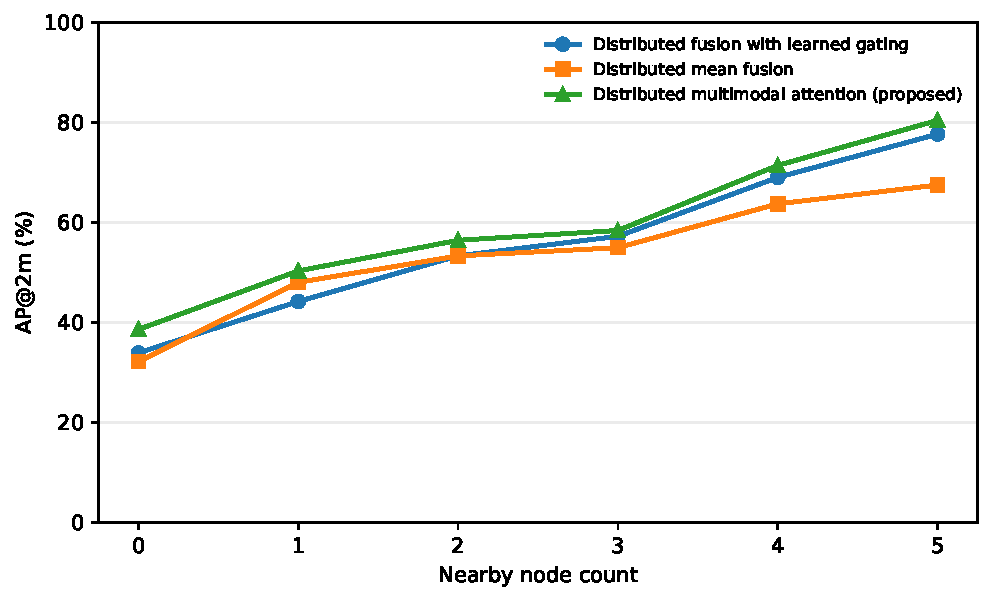
\includegraphics[width=0.90\textwidth]{paper_results/figures/fig_01_node_count_ap.pdf}
    \caption{AP@2m as the number of available nearby sensing nodes varies.}
    \label{fig:experiments-node-ap}
\end{figure}

\begin{figure}[H]
    \centering
    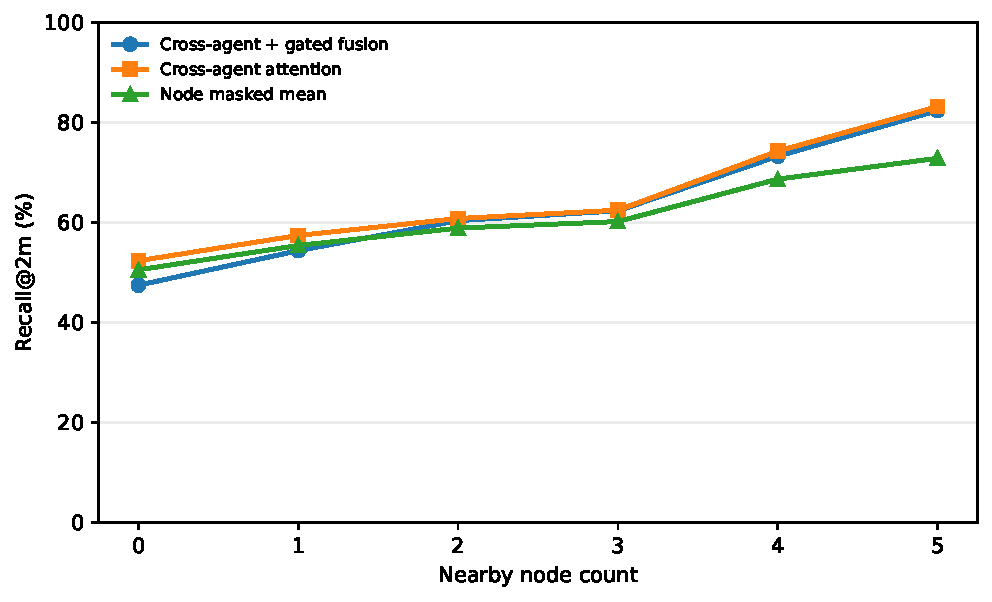
\includegraphics[width=0.90\textwidth]{paper_results/figures/fig_02_node_count_recall.pdf}
    \caption{Recall@2m as the number of available nearby sensing nodes varies.}
    \label{fig:experiments-node-recall}
\end{figure}

\begin{figure}[H]
    \centering
    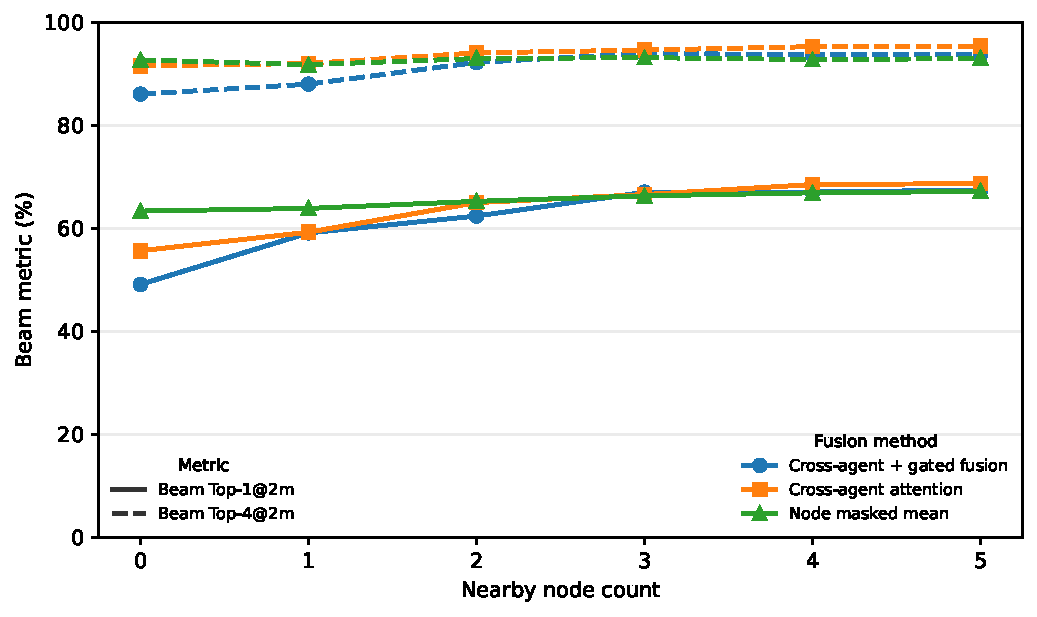
\includegraphics[width=0.90\textwidth]{paper_results/figures/fig_03_node_count_beam.pdf}
    \caption{Beam Top-1@2m and Top-4@2m as the number of available nearby
    sensing nodes varies.}
    \label{fig:experiments-node-beam}
\end{figure}

\section{Communication Performance}
\label{sec:experiments-beam-management}

\subsection{Performance Across Environmental Conditions}
\label{subsec:experiments-weather-system}

Table~\ref{tab:experiments-system-weather} and
Figure~\ref{fig:experiments-weather-rate} compare the three measurement
policies under each environmental condition.  In Clear conditions, DMSA-BM
reaches an effective user rate of \(155.453\) Mbps with \(1.39\%\) CSI-RS
overhead.  SSB-guided refinement with \(K_{\mathrm{ref}}=4\) reaches
\(151.367\) Mbps with \(1.90\%\) overhead, whereas the
\(K_{\mathrm{ref}}=12\) operating point reaches \(127.033\) Mbps with
\(5.71\%\) overhead.

The sensing-use entries and their complementary fallback ratios clarify how
the policy reaches these outcomes.  Sensing candidates are used for \(76.35\%\)
of the Clear instances, \(56.65\%\) of the Rain/Fog instances, and \(30.07\%\)
of the Night instances.  The corresponding fallback ratios are \(23.65\%\), \(43.35\%\), and
\(69.93\%\).  Thus, DMSA-BM retains SSB-guided refinement whenever no
accepted association with a currently observed track is available, instead of
applying target-indexed beam information to a VUE unconditionally.

\begin{table}[H]
    \centering
    \caption{Communication performance by environmental condition under the
    common system configuration.  The effective rate is averaged over VUEs and
    communication cycles.}
    \label{tab:experiments-system-weather}
    \small
    \renewcommand{\arraystretch}{1.10}
    \resizebox{\textwidth}{!}{%
    \begin{tabular}{llrrr}
        \toprule
        Condition & Policy & Effective rate (Mbps) &
        CSI-RS overhead (\%) & Sensing use (\%) \\
        \midrule
        Clear & SSB-guided refinement, \(K_{\mathrm{ref}}=4\) & 151.367 & 1.90 & 0.00 \\
        Clear & SSB-guided refinement, \(K_{\mathrm{ref}}=12\) & 127.033 & 5.71 & 0.00 \\
        Clear & DMSA-BM & 155.453 & 1.39 & 76.35 \\
        \addlinespace
        Rain/Fog & SSB-guided refinement, \(K_{\mathrm{ref}}=4\) & 147.571 & 1.90 & 0.00 \\
        Rain/Fog & SSB-guided refinement, \(K_{\mathrm{ref}}=12\) & 115.342 & 5.71 & 0.00 \\
        Rain/Fog & DMSA-BM & 150.801 & 1.57 & 56.65 \\
        \addlinespace
        Night & SSB-guided refinement, \(K_{\mathrm{ref}}=4\) & 127.807 & 1.90 & 0.00 \\
        Night & SSB-guided refinement, \(K_{\mathrm{ref}}=12\) & 105.294 & 5.71 & 0.00 \\
        Night & DMSA-BM & 132.743 & 1.71 & 30.07 \\
        \bottomrule
    \end{tabular}%
    }
\end{table}

\begin{figure}[H]
    \centering
    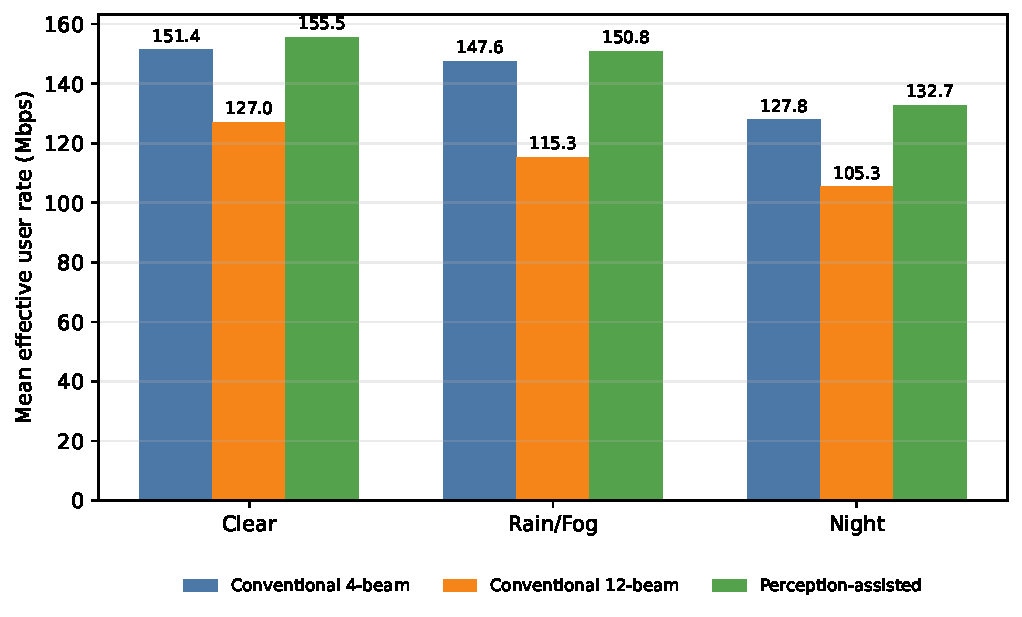
\includegraphics[width=0.88\textwidth]{paper_results/figures/fig_04_core_user_rate_by_weather.pdf}
    \caption{Effective user rate by environmental condition and measurement
    policy.}
    \label{fig:experiments-weather-rate}
\end{figure}

\subsection{Aggregate Performance}
\label{subsec:experiments-macro-system}

Figure~\ref{fig:experiments-system-tradeoff} aggregates the three environmental
conditions with equal weight.  DMSA-BM achieves an effective user rate of
\(146.332\) Mbps with \(1.56\%\) CSI-RS overhead.  The corresponding values
for SSB-guided refinement are \(142.248\) Mbps and \(1.90\%\) at
\(K_{\mathrm{ref}}=4\), and \(115.890\) Mbps and \(5.71\%\) at
\(K_{\mathrm{ref}}=12\).

DMSA-BM remains explicitly conditional.  Its aggregate sensing-use ratio is
\(54.35\%\), while \(45.65\%\) of instances use SSB-guided refinement as the
fallback.  Taken together, the rate and overhead values show
the consequence of using sensing only when a current detection and a credible
target-to-user association are available.  The service beam is still selected
from the actually measured CSI-RS candidates.

\begin{figure}[H]
    \centering
    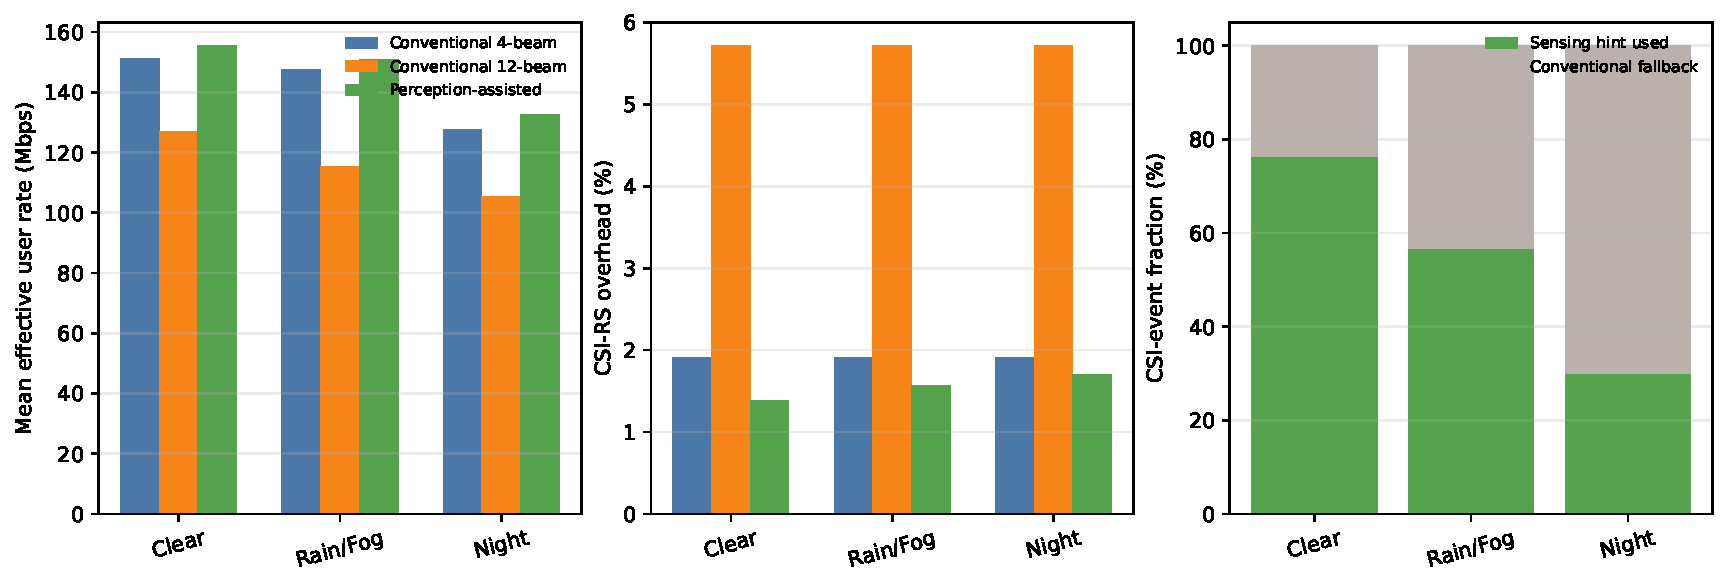
\includegraphics[width=0.96\textwidth]{paper_results/figures/fig_05_core_user_rate_hint_overhead.pdf}
    \caption{Aggregate effective rate, CSI-RS overhead, and the
    sensing-use/fallback composition under the common system configuration.}
    \label{fig:experiments-system-tradeoff}
\end{figure}

\section{Tracking Performance}
\label{sec:experiments-tracking}

\subsection{Comparison of Tracking Models}
\label{subsec:experiments-tracker-system}

Table~\ref{tab:experiments-trackers} evaluates the three trackers with the same
Top-1 CE detector and system configuration.  Their effective rates are close,
with \(146.332\) Mbps for IMM, \(146.373\) Mbps for KF-CV, and
\(145.880\) Mbps for KF-CT.  KF-CV is marginally higher than IMM in this
metric.  The table therefore does not support an effective-rate claim of
universal IMM superiority.

The sensing-use ratios are also close, at \(54.35\%\) for IMM, \(53.80\%\) for
KF-CV, and \(52.26\%\) for KF-CT.  These values show that the three trackers
operate at comparable frequencies of sensing-assisted candidate selection under
the evaluated procedure.  IMM is retained in DMSA-BM for its
multi-model state-estimation role in association maintenance.  The table should
therefore be interpreted as an end-to-end comparison rather than as a
tracker-only proof of superiority.

\begin{table}[H]
    \centering
    \caption{Aggregate communication results for the tracker variants under
    the common detector and system configuration.}
    \label{tab:experiments-trackers}
    \small
    \begin{tabular}{lrr}
\toprule
Tracker & Mean effective user rate (Mbps) & Sensing use (\%) \\
\midrule
IMM & 146.332 & 54.35 \\
KF-CV & \textbf{146.373} & 53.80 \\
KF-CT & 145.880 & 52.26 \\
\bottomrule
\end{tabular}

\end{table}

\section{Discussion and Limitations}
\label{sec:experiments-discussion}

The results support a consistent evidence chain.  Multimodal and nearby-node
observations improve different aspects of target availability and beam ranking;
association acceptance and current-track observation determine whether this
evidence is converted into a narrower CSI-RS measurement action; and the system
evaluation reports the resulting effective throughput together with the
associated measurement cost.  The substantial fallback share under Rain/Fog
and Night is therefore an integral part of DMSA-BM and should be interpreted
together with the average-rate result.

The system analysis characterises association-mediated operation through the
sensing-use ratio, fallback ratio, and average effective user rate; accepted-association
accuracy, lower-tail rate, and outage are outside the reported analysis.  The
conclusions are further limited to a local target-BS service region, a simulated
multimodal dataset, approximately 100-ms ray-tracing channel segments, and the
stated RZF and resource model.  They therefore describe performance under the
specified system assumptions rather than a complete 5G NR protocol stack or a
direct real-world deployment.

\chapter{Conclusion and Future Work}
\label{ch:conclusion}

\section{Conclusion}
\label{sec:conclusion-summary}

This thesis studied multimodal sensing-assisted user association and tracking
for beam management in vehicular networks. The motivating problem is that
vehicle users in road-side communication scenarios experience rapidly changing
geometry, blockage, and beam quality, while repeated beam sweeping and channel
measurement can consume non-negligible radio resources. To address this
setting, the thesis considered a BS-centric sensing infrastructure in which the
serving base station (BS) and nearby sensing nodes (SNs) provide multiview
camera observations, and the BS also provides an ISAC point cloud. These
observations are organised through a bird's-eye-view (BEV) representation so
that vehicle detection, per-target beam prediction, and communication-oriented
evaluation can be studied within a common spatial frame.

The first part of the work formulated a multimodal distributed
sensing-assisted beam management framework. In this framework, camera modality
and ISAC modality are fused in BEV space to detect vehicle targets and estimate
per-target beam-class posteriors. The resulting ranked Top-K candidate beams
provide a sensing-driven interface between the perception system and the subsequent
communication evaluation. The objective of this design is not to replace
communication measurements entirely, but to use sensing observations to reduce
the frequency and scope of expensive beam measurements when the sensing output
is sufficiently reliable.

The second part of the work addressed the identity mismatch between sensing
targets and communication users. Since a detected vehicle target is not
automatically associated with a communication user identity, the proposed
workflow uses the initial SSB beam sweep power spectrum to establish
target-user association. After this initial binding, an interacting multiple
model (IMM) tracking process maintains the temporal continuity of vehicle
states and supports beam maintenance in subsequent frames. This association and
tracking layer is central to the thesis scope because it connects per-frame
sensing predictions with a persistent communication service process.

The third part of the work specified a multimodal simulation and system-level
evaluation methodology. The evaluation connects road traffic
simulation, multiview sensing data generation, ISAC-like point clouds,
ray-tracing-based beam labels, and simplified communication metrics. Within
this abstraction, beam prediction accuracy, target-user association, tracking
quality, beam training overhead, beam mismatch, zero-forcing (ZF) precoding
SINR, spectral efficiency, and overhead-adjusted throughput can be considered
together. This evaluation pipeline makes explicit how errors in sensing and
identity maintenance may propagate into communication-level performance.
The overall contribution is therefore a framework-level and evaluation-level
study of multimodal sensing-assisted beam management rather than a
protocol-complete 5G NR implementation.

\section{Limitations}
\label{sec:conclusion-limitations}

Several limitations follow from the current scope of the thesis. First, the
evaluation relies on a simulated or generated multimodal
environment. Such a setting is necessary for controlled access to camera
observations, ISAC-like point clouds, vehicle trajectories, beam labels, and
channel data, but it may introduce a domain gap relative to real road-side
deployments. The appearance of vehicles, sensing noise, calibration quality,
traffic behaviour, occlusion patterns, and propagation conditions in real
networks may differ from those represented by the simulation pipeline.

Second, the communication evaluation is a simplified and interpretable
abstraction rather than a complete 5G NR protocol stack. The thesis models
beam management, beam mismatch, ZF precoding SINR, spectral efficiency, and
overhead-adjusted throughput at a system level, but it does not fully model
protocol-level details such as SSB and CSI-RS scheduling, feedback latency,
control signaling, HARQ behaviour, scheduler interaction, or mobility management
procedures. As a result, throughput-related quantities should be interpreted as
evaluation indicators under the stated abstraction, not as direct predictions
of deployment-level 5G NR performance.

Third, the proposed sensing-assisted workflow depends on the reliability of
multimodal sensing and cross-modal alignment. Camera calibration errors,
time-synchronization errors, sparse or noisy ISAC point clouds, missing
modalities, and severe occlusion can degrade BEV detection, beam prediction,
target-user association, and tracking. The framework includes partial beam
measurement and re-association as possible recovery mechanisms, but the precise
robustness limits and failure thresholds remain important factors for
system-level evaluation and deployment-oriented future work.

Fourth, the thesis focuses primarily on a BS-centric local service region.
This choice keeps the problem tractable and allows the relationship between
multimodal sensing, target-user association, tracking, and beam management to
be studied clearly. However, it leaves broader network-level questions only
partially addressed, including cooperative multi-BS beam management,
inter-cell interference, load-aware service selection, and handover decisions
for vehicles moving across BS coverage regions.

\section{Future Work}
\label{sec:conclusion-future-work}

Future work should extend the thesis in directions that directly correspond to
the limitations above.

\subsection{Real-World Deployment and Domain Gap}
\label{subsec:future-domain-gap}

A natural next step is to evaluate the framework with real road-side sensing
and communication data. This may include collecting synchronized multiview
camera observations, ISAC or radar-like point clouds, vehicle trajectories, and
communication beam measurements from instrumented road-side infrastructure.
Such data would make it possible to quantify the domain gap between simulation
and deployment, validate the assumptions used in the BEV fusion pipeline, and
study whether synthetic-to-real adaptation is necessary for reliable beam
prediction and target-user association.

\subsection{Protocol-Level 5G NR Simulation}
\label{subsec:future-5g-nr}

The communication abstraction can be extended toward a fuller 5G NR
protocol-level simulation. Future work may incorporate more detailed modelling
of SSB and CSI-RS timing, beam reporting, feedback delay, scheduling, control
overhead, retransmission behaviour, and mobility procedures. This would allow
sensing-assisted beam management to be evaluated not only through simplified
SINR and throughput indicators, but also through protocol-aware latency,
resource utilization, and service continuity metrics.

\subsection{Online and Domain Adaptation}
\label{subsec:future-online-adaptation}

The present framework is primarily described as an offline trained and
evaluated system. Future work can investigate online adaptation so that the
beam prediction, association, and tracking modules can adjust to new roads,
sensor placements, vehicle distributions, and propagation conditions. Possible
directions include continual calibration, self-supervised adaptation from
communication measurements, and domain adaptation between simulated and real
scenarios. These extensions should be designed carefully to avoid reinforcing
incorrect associations or unreliable beam predictions during deployment.

\subsection{Cooperative Multi-BS Beam Management and Handover}
\label{subsec:future-multi-bs-handover}

Finally, the BS-centric design can be extended to cooperative multi-BS beam
management and handover. In a multi-BS network, sensing and tracking states may
be shared across neighboring BSs to support service-BS selection, handover
preparation, and coordinated beam decisions for fast-moving vehicles. This
extension would require new association variables linking vehicles, sensing
tracks, serving BSs, and candidate beams, as well as evaluation metrics that
capture handover reliability, inter-cell coordination overhead, and service
continuity.


%% -------------------------------------------------
%% References
%% -------------------------------------------------

\printbibliography[heading=bibintoc,title=References]

%% -------------------------------------------------
%% Appendices
%% -------------------------------------------------
\appendix

\chapter{List of Publications}
\label{app:publications}

\paperlist[Conference Papers]{LoP.YuanVTC2025}

\chapter{Additional Requirements}
\label{app:requirements}

TODO: Add program-specific or formatting-related appendix content if required.



\end{document}
